%%%%%%%%%%%%%%%%%%%%%%%%%%%%%%%%%%%%%%%%%%%%%%%%%%%%%%%%%%%%%%%%%%%%
%% I, the copyright holder of this work, release this work into the
%% public domain. This applies worldwide. In some countries this may
%% not be legally possible; if so: I grant anyone the right to use
%% this work for any purpose, without any conditions, unless such
%% conditions are required by law.
%%%%%%%%%%%%%%%%%%%%%%%%%%%%%%%%%%%%%%%%%%%%%%%%%%%%%%%%%%%%%%%%%%%%

\documentclass[
  digital,     %% The `digital` option enables the default options for the
               %% digital version of a document. Replace with `printed`
               %% to enable the default options for the printed version
               %% of a document.
%%  color,       %% Uncomment these lines (by removing the %% at the
%%               %% beginning) to use color in the printed version of your
%%               %% document
  oneside,     %% The `oneside` option enables one-sided typesetting,
               %% which is preferred if you are only going to submit a
               %% digital version of your thesis. Replace with `twoside`
               %% for double-sided typesetting if you are planning to
               %% also print your thesis. For double-sided typesetting,
               %% use at least 120 g/m² paper to prevent show-through.
  nosansbold,  %% The `nosansbold` option prevents the use of the
               %% sans-serif type face for bold text. Replace with
               %% `sansbold` to use sans-serif type face for bold text.
  nocolorbold, %% The `nocolorbold` option disables the usage of the
               %% blue color for bold text, instead using black. Replace
               %% with `colorbold` to use blue for bold text.
  nolof,         %% The `lof` option prints the List of Figures. Replace
               %% with `nolof` to hide the List of Figures.
  nolot,         %% The `lot` option prints the List of Tables. Replace
               %% with `nolot` to hide the List of Tables.
]{fithesis4}
%% The following section sets up the locales used in the thesis.
\usepackage[resetfonts]{cmap} %% We need to load the T2A font encoding
\usepackage[T1,T2A]{fontenc}  %% to use the Cyrillic fonts with Russian texts.
\usepackage[
  main=english, %% By using `czech` or `slovak` as the main locale
                %% instead of `english`, you can typeset the thesis
                %% in either Czech or Slovak, respectively.
  english, german, russian, czech, slovak %% The additional keys allow
]{babel}        %% foreign texts to be typeset as follows:
%%
%%   \begin{otherlanguage}{german}  ... \end{otherlanguage}
%%   \begin{otherlanguage}{russian} ... \end{otherlanguage}
%%   \begin{otherlanguage}{czech}   ... \end{otherlanguage}
%%   \begin{otherlanguage}{slovak}  ... \end{otherlanguage}
%%
%% For non-Latin scripts, it may be necessary to load additional
%% fonts:
\usepackage{paratype}
\usepackage{todonotes}
\setuptodonotes{inline}
\def\textrussian#1{{\usefont{T2A}{PTSerif-TLF}{m}{rm}#1}}
%%
%% The following section sets up the metadata of the thesis.
\thesissetup{
    date        = \the\year/\the\month/\the\day,
    university  = mu,
    faculty     = fi,
    type        = bc,
    department  = Department of Computer Systems and Communications,
    author      = Tomáš Marek,
    gender      = f,
    advisor     = {Ing. Milan Brož, Ph.D.},
    title       = {Improvements of the Randomness Testing Toolkit},
    TeXtitle    = {Improvements of the Randomness Testing Toolkit},
    keywords    = {keyword1, keyword2, ...},
    TeXkeywords = {keyword1, keyword2, \ldots},
    abstract    = {%
      This is the abstract of my thesis, which can

      span multiple paragraphs.
    },
    thanks      = {%
      These are the acknowledgements for my thesis, which can

      span multiple paragraphs.
    },
    bib         = bibliography.bib,
    %% Remove the following line to use the JVS 2018 faculty logo.
    facultyLogo = fithesis-fi,
}
\usepackage{makeidx}      %% The `makeidx` package contains
\makeindex                %% helper commands for index typesetting.
%% These additional packages are used within the document:
\usepackage{paralist} %% Compact list environments
\usepackage{amsmath}  %% Mathematics
\usepackage{amsthm}
\usepackage{amsfonts}
\usepackage{url}      %% Hyperlinks
\usepackage{markdown} %% Lightweight markup
\usepackage{listings} %% Source code highlighting
\lstset{
  basicstyle      = \ttfamily,
  identifierstyle = \color{black},
  keywordstyle    = \color{blue},
  keywordstyle    = {[2]\color{cyan}},
  keywordstyle    = {[3]\color{olive}},
  stringstyle     = \color{teal},
  commentstyle    = \itshape\color{magenta},
  breaklines      = true,
}
\usepackage{floatrow} %% Putting captions above tables
\floatsetup[table]{capposition=top}
\usepackage[babel]{csquotes} %% Context-sensitive quotation marks
\begin{document}
%% The \chapter* command can be used to produce unnumbered chapters:
\chapter*{Introduction}
%% Unlike \chapter, \chapter* does not update the headings and does not
%% enter the chapter to the table of contents. I we want correct
%% headings and a table of contents entry, we must add them manually:
\markright{\textsc{Introduction}}
\addcontentsline{toc}{chapter}{Introduction}

% RANDOMNESS TESTING - 'theoretical' chapter

\chapter{Randomness testing}

\section{Overview / Introduction}

%Random number generators are tested by taking an output sample. This 
%Testing a sequence (define) (tu01guide - 1, tu01paper - 3, 17), required properties(nistspecial 1-1, 1-3 )


During a randomness test a \emph{random sequence} is tested. In this document, a random sequence is a finite sequence of zero and one bits, which was generated by a tested source of randomness. The desired properties of random sequence are \emph{uniformity} (for each bit the probability for both zero and one are exactly $1/2$), \emph{independence} (none of the bits is influenced by any other bit) and \emph{unpredictability} (it is impossible to predict next bit by obtaining any number of previous bits). \cite[p. 1-1]{nist_special}

%Null/alternative hypothesis (tu01paper - 3, možná učebnice)
%Randomness testing as statistical testing (tu01guide - 2)

Randomness test is a form of \emph{empirical statistical test}, where we test our assumption about the tested data - the \emph{null hypothesis} ($H_0$). During the randomness test it states that the sequence is \emph{random}. Associated with the null-hypothesis is the \emph{alternative hypothesis} ($H_1$), which states that the sequence is \emph{nonrandom}. Goal of the test is to search for evidence against the null-hypothesis. \cite[p. 2]{tu01_guide}

%Idea of testing – extremeness of a sample ? (nistspecial - 1-3+)

%result (accept, reject, Type I/II error) (nistspecial - 1-3+, učebnice 416)

The result of the test is either that we \emph{accept} the null hypothesis (the sequence is considered random), or that we \emph{reject} the null-hypothesis (and accept the alternative hypothesis - the sequence is considered nonrandom). We reject the null hypothesis when the evidence found against the null-hypothesis is strong, otherwise we accept it. Based on the true situation of null hypothesis, four situations depicted in Table \ref{tab:type_errors} may occur. \cite[p. 417]{basic_practice}

\begin{table}
  \begin{tabularx}{0.7\textwidth}{l|c|c}
    %\toprule
    TRUE  & \multicolumn{2}{c}{TEST CONCLUSION}\\
    SITUATION &Accept $H_0$ & Reject $H_0$\\
    \midrule
    $H_0$ is True &  No error & Type I error  \\
    $H_0$ is False & Type II error & No error \\
    %\bottomrule
  \end{tabularx}
  \caption{Possible outcomes when assessing the result of statistical test.}
  \label{tab:type_errors}
\end{table}

\section{One-level testing}

%significance level (tu01 paper 5-8, nistspecial 1-3+, rec for stat testing 5, učebnice)

The \emph{significance level} ($\alpha$) must be set for the test. The $\alpha$ is equal to probability of Type I Error. Usual values are $\alpha = 0.05$ or $\alpha = 0.01$ \cite[p. 390]{basic_practice}, for use in testing of cryptographic random number generators lower values may be chosen. \cite[p. 1-4]{nist_special} The lower $\alpha$ is set, the stronger the found evidence has to be to reject the null hypothesis. (cite? derived from nistspecial 1-4)

%Test statistic (= function, known distribution), sample (tu01 paper 4+)

The randomness test is defined by a \emph{test statistic} $Y$, which is a function of a finite bit sequence. Distribution of its values under the null hypothesis must be known (or at least approximated). The value of the test statistic ($y$) is computed for the tested random sequence. Each test statistic searches for presence or absence of some "pattern" in the sequence, which would show the nonrandomness of the sequence. There is infinite number of possible test statistics. \cite[p. 4]{tu01_paper}

%p-value (one, two tailed, how extremeness is set) (nist-opt 5, nist-special 1-4,rec for stat testing 5)

The \emph{p-value} of the test is the probability of the test statistic $Y$ taking value at least as extreme as the observed $y$, assuming that the null hypothesis is true. In randomness testing it is equal to the probability that \emph{perfect random generator} would generate less random sequence. The smaller is the p-value, the stronger is the found evidence against the null-hypothesis. \cite[p. 386]{basic_practice} The p-value is calculated based on the observed $y$.



\subsection{Result interpretation}
%interpratation (učebnice 380-400)

Decision about the test result is based on the computed \emph{p-value}. If the p-value is lower than the $\alpha$, we \emph{reject the null hypothesis} (and accept the alternative hypothesis), because strong enough evidence against randomness was found. If the p-value is greater than or equal to the $\alpha$, we \emph{accept the null hypothesis}, because the evidence against the null hypothesis was too weak. \cite[p. 390]{basic_practice} It is often recommended to report the \emph{p-value} as well instead of accept/reject only, as it yields more information. \cite[p. 90]{tu01_guide}

% TODO: note on moving alpha, for one alpha fail, for other pass

The p-values close to $\alpha$ can be considered \emph{suspicious}, because they do not clearly indicate rejection. Further testing of the random number generator on \emph{other} random sequences is then in place to search for further evidence. \cite[p. 5]{tu01_paper} The reason is that \emph{randomness} is a probabilistic property, therefore even the perfect random number generator may generate a nonrandom sequence with low p-value (although it is very unlikely). The further evidence is used to differentiate between the bad generator generating a nonrandom sequence systematicaly and the good generator generating nonrandom sequence 'by chance'. \cite[p. 90]{tu01_guide}




\todo{REWRITE}
%example
\subsection{Example} \label{chap:rand-example}


To demonstrate how a single randomness test is made, the Frequency (Monobit) Test from NIST STS battery was chosen. \cite[p. 2-2]{nist_special} This test is based on testing the fraction of zeroes and ones within the sequence. For a random sequence with length $n$ the  count of ones (and zeroes) is expected to be around $n/2$ (i.e. the most probable values are close to $n/2$). 

It is easy to see that with one of the counts increasing (and the second one therefore decreasing), the sequence is getting less random. The probability of the bit being zero or one shifts from both being equal in favor of the more frequent bit.

For the Monobit test it is recommended for the tested sequence to have at least 100 bits. The test statistic $S_{obs}$ of the Monobit test is defined as \[S_{obs} = \dfrac{|\#_1 - \#_0|}{\sqrt{n}}\] where $\#_1$ is count of ones in the tested sequence (similarly for zeroes) and $n$ is length of of the tested sequence. Under the null hypothesis, the reference distribution of $S_{obs}$ is half normal (for large $n$). 

The p-value is computed as \[ p = erfc(\dfrac{S_{obs}}{\sqrt{2}}) \] where $erfc$ is the \emph{complementary error function} used to calculate probabilities in normal distribution.

 Let
\[\begin{split}
    \epsilon = 10011001010010000010001001011001101100001101000111\\10101001010010010011100111001100110010010100111011
\end{split}\]
 be the tested sequence. The test statistic for this sequence is 

 \[S_{obs} = \dfrac{|46 - 54|}{\sqrt{100}}\ = \dfrac{|-8|}{10} = 0.8\]
 and the p-value (visualised at Figure \ref{fig:example}) is 
 \[p = erfc\biggl(\dfrac{0.8}{\sqrt{2}}\biggr) \approx 0.423\]

To interpret the test, we compare the computed \emph{p-value} to the chosen $\alpha$. Since the $\emph{p-value} \approx 0.423$ is greater than both usual $\alpha = 0.05$ and $\alpha = 0.01$, we accept the null hypothesis for both \emph{significance levels}. Therefore, the sequence $\epsilon$ is considered random.

\begin{figure}
  \begin{center}
    %% minimus is about 100 pixels per 1 centimeter or 300 pixels per 1 inch.
    %% The optimum is about 250 pixels per 1 centimeter 
    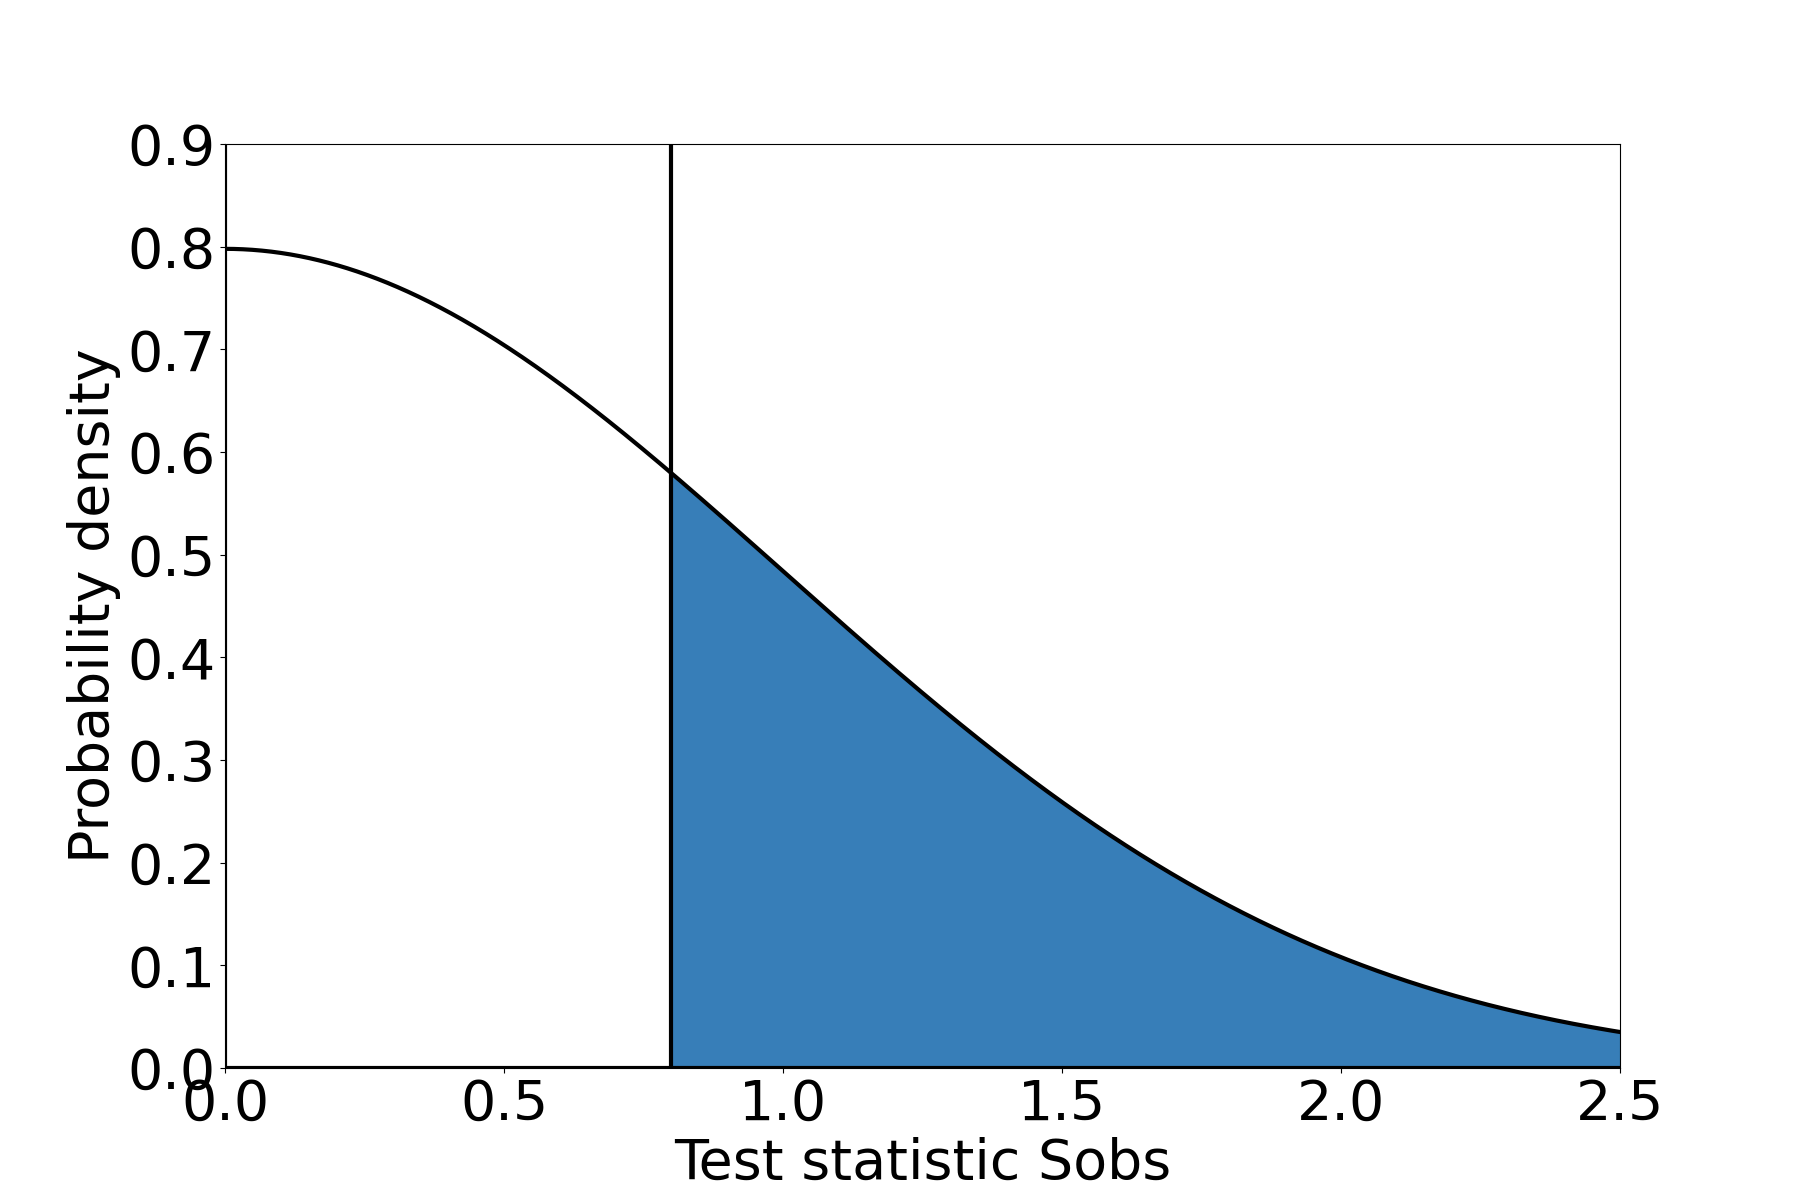
\includegraphics[width=8cm]{figures/test_example.png}
  \end{center}
  \caption{Visualization of example p-value}
  \label{fig:example}
\end{figure}

 



\section{Two level testing} \label{chap:rand-two_level}

TODO: mention expected fails of of first levels, figure with schema, mention remaining GOF tests


Two-level testing is used for a further examination of the data and can yield stronger information than using a one-level testing only. . 

To perform a two level test, we split the original sequence into $n$ equal length non-overlapping sequences. Then we perform a standard statistical test as described in Section \ref{chap:rand-process} on each of these sequences in separate and collect all of the p-values they generated. These tests are then called first-level tests and their respective p-values are called first-level p-values. 

Note that the first-level p-values are not interpreted at this moment. It is in fact expected that some first-level p-values will be lower than the chosen \emph{significance level} (these would usually be considered failed). Given that the null hypothesis is true, the number of 'failed' first-level tests is expected to be $\alpha\cdot100\%$ of the total number of first-level p-values.

The first-level p-values are only treated as data in second round of testing, where goodness of fit tests are used - the second-level test. The goodness-of-fit tests are used to determine how well the observed data fit expected distribution. The most notable examples of tests from this category are the Kolmogorov-Smirnov test and the $\chi^2$ test, another examples are Cramér-von Mises test and Anderson-Darling test. 

For the first-level p-values a uniform distribution with interval $<0,1>$ is expected. The second-level test yields one second-level p-value, which is interpreted the same way a one-level test p-value would be (as described in Subsection \ref{chap:rand-interpretation}). Several goodness of fit tests can be applied at the same set of first-level p-values at once, because each test examines different uniformity properties of the data.

TODO: DIG DEEPER INTO DIFFERENCES BETWEEN GOF TESTS

% KS - description
\subsection{Kolmogorov-Smirnov test}
There are two variants of the Kolmogorov-Smirnov test (KS test). Two-sample test is used for comparing distributions of two data samples (to check if the data samples share the same distribution). The second variant, which is used in randomness testing, is the one-sample test. The one-sample test is used to compare a data sample against a theoretical distribution.

The Kolmogorov-Smirnov test is based on comparing the cumulative distribution function (CDF) of the expected distribution and the empirical cumulative distribution function (eCDF) of the observed samples. The Kolmogorov-Smirnov ($D$) statistic is the maximal absolute difference (vertical distance) between the expected CDF and observed eCDF (as can be seen in Figure \ref{fig:ks_d}). In some variants of the Kolmogorov-Smirnov test two statistics are measured - the maximal distance above the CDF ($D^+$) and the maximal distance below the CDF ($D^-$). Once the statistic is obtained, the second-level p-value is computed. Formally, the test statistics are defined as
\[\begin{split}
    &D^+ = sup_x\{F_n(x) - F(x)\}\\
    &D^- = sup_x\{F(x) - F_n(x)\}\\
    &D \:\:\:= sup_x\{|F_n(x) - F(x)|\} = max(D^+, D^-)
\end{split}
\] where $F(x)$ is the CDF and $F_n(x)$ is the  eCDF \cite[p. 100]{GOF-techniques}.

\begin{figure}
  \begin{center}
    %% minimus is about 100 pixels per 1 centimeter or 300 pixels per 1 inch.
    %% The optimum is about 250 pixels per 1 centimeter 
    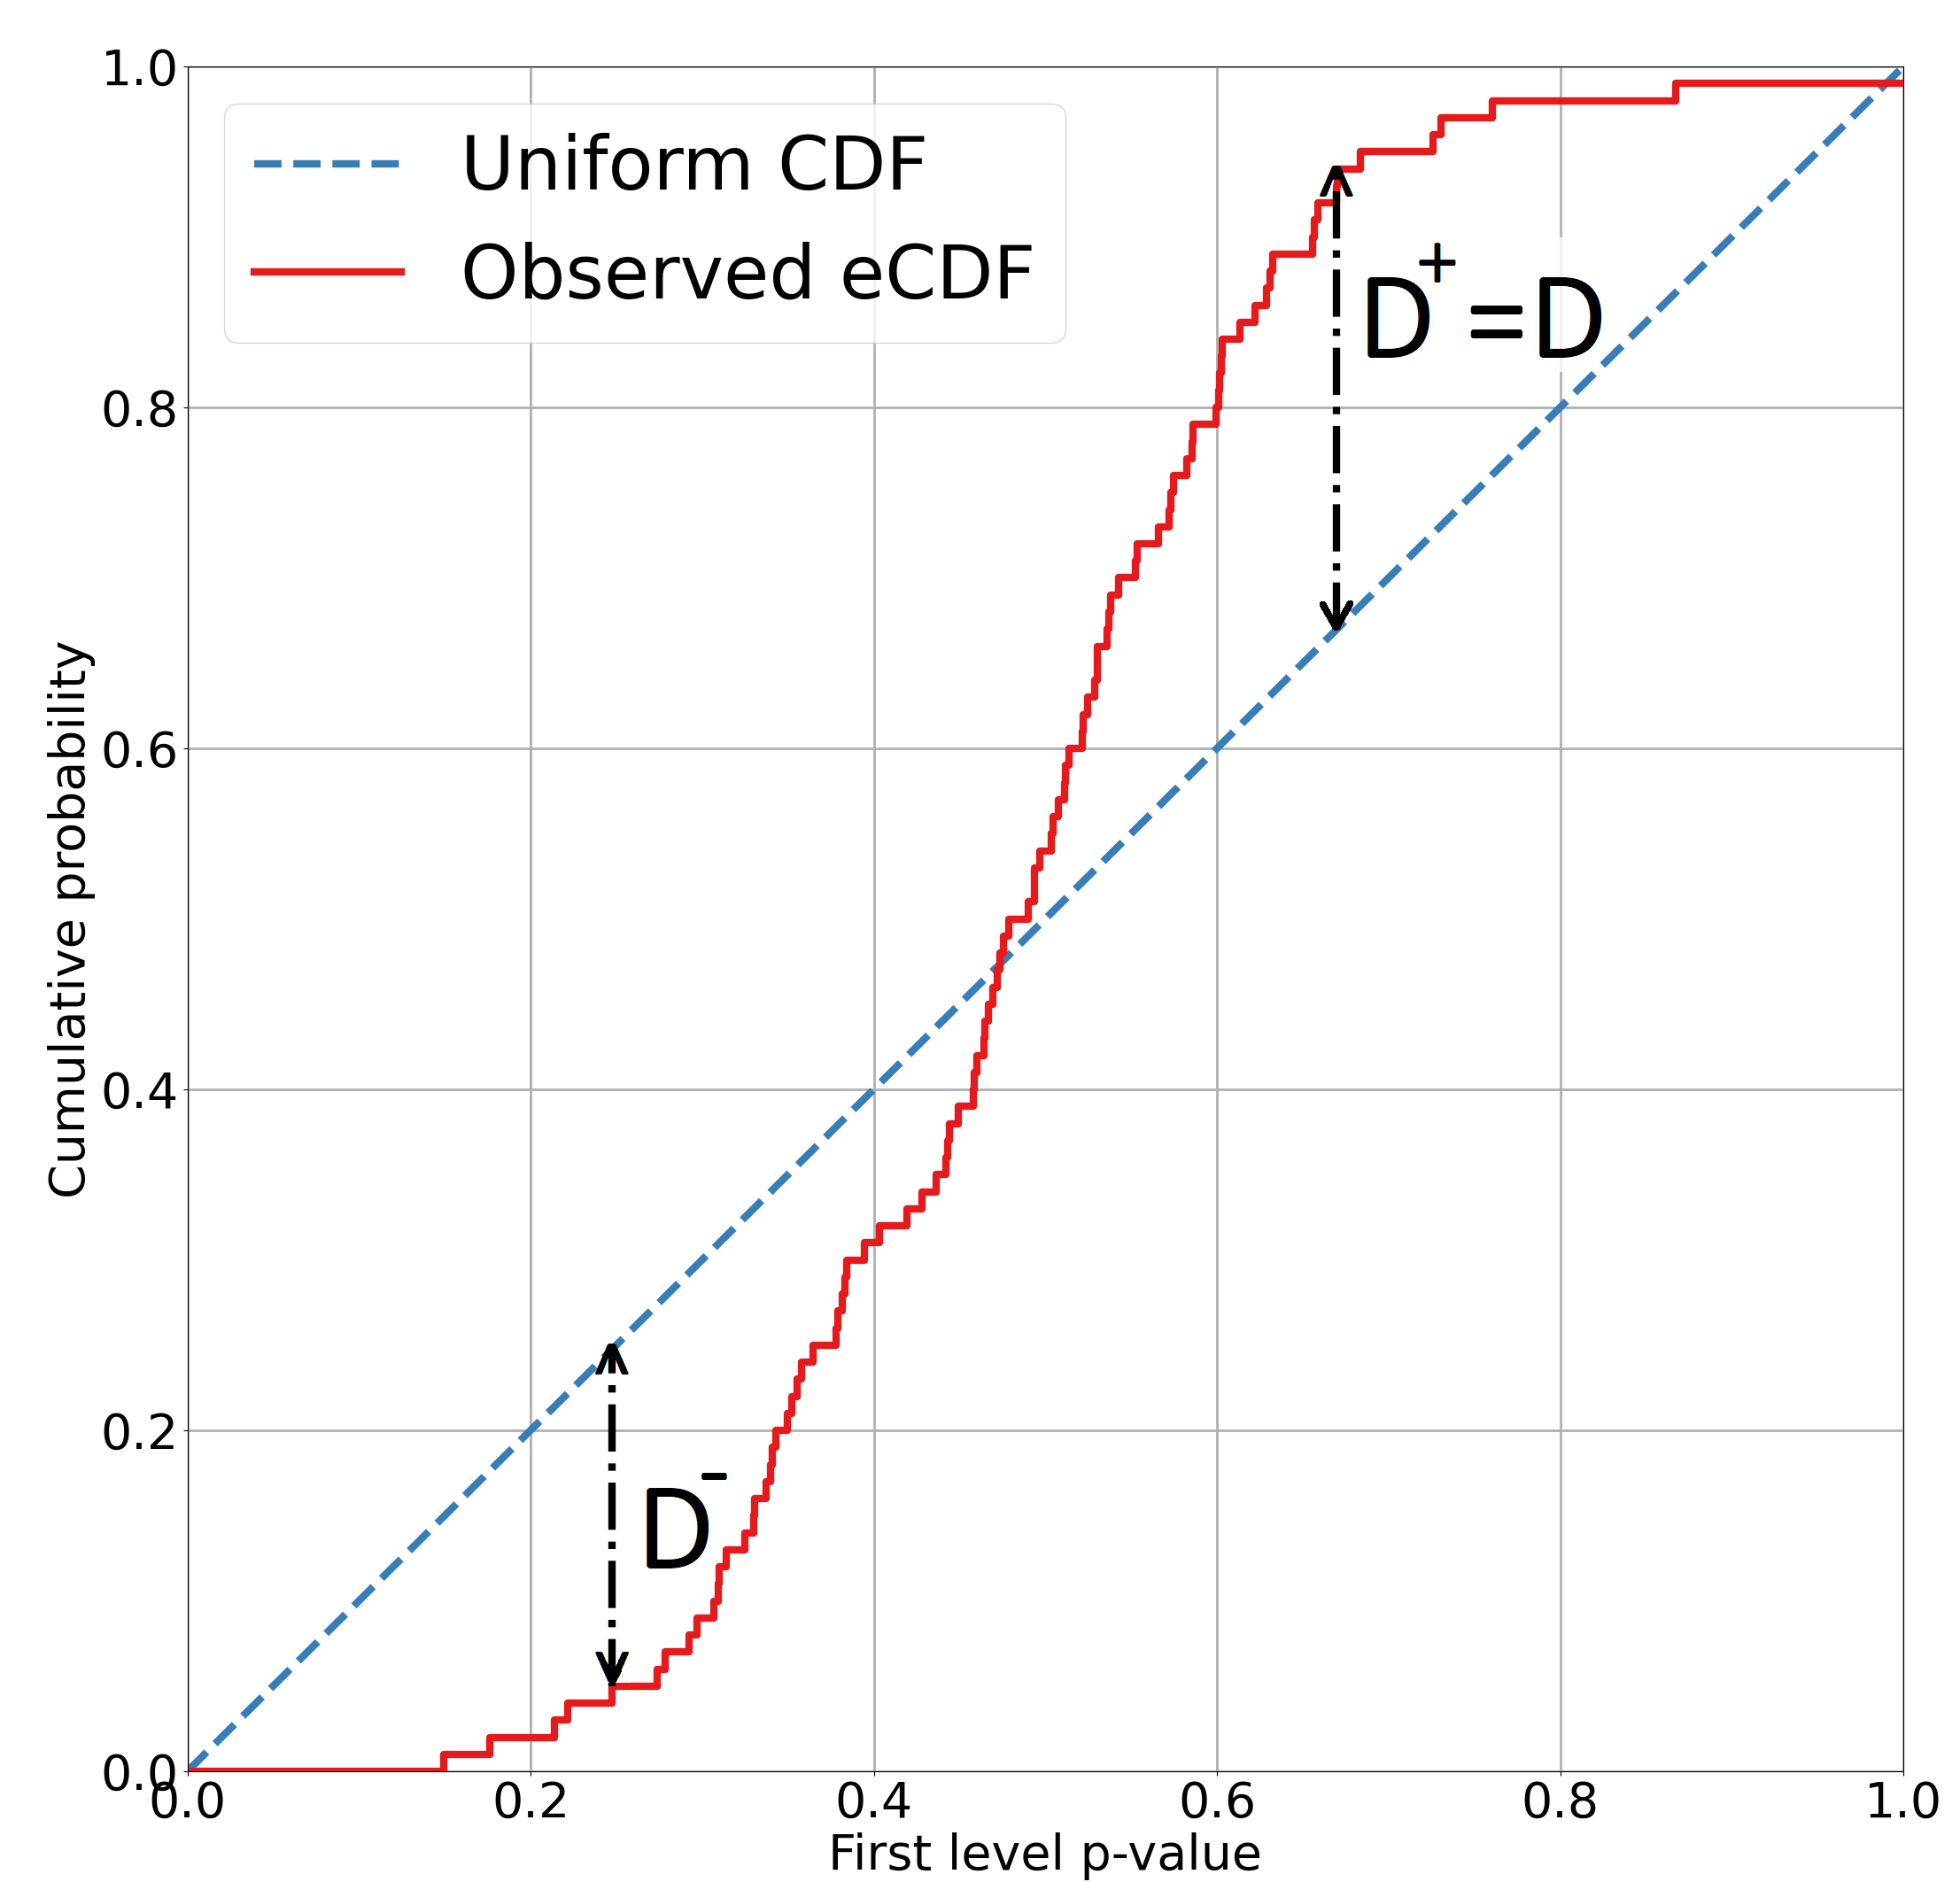
\includegraphics[width=8cm]{figures/ks_d.png}
  \end{center}
  \caption{Kolmogorov-Smirnov test statistics}
  \label{fig:ks_d}
\end{figure}


% $\chi^2$ description
\subsection{$\chi^2$ test}
$\chi^2$ tests are a group of several statistical tests used for comparing two sets of categorical data. The main one is the Pearson's $\chi^2$ test, that is used to determine existence of statistically significant difference in frequencies of categories in data sets. In randomness testing, one data set are the observed first-level p-values that are divided into $n$ equal-width categories and their respective frequencies are counted. The second data set are the expected frequencies for each category. Because the expected distribution of p-values is uniform, the expected frequencies are equal in each category. 
 
The test is based on summing squared differences in frequencies for each category between both sets of data. For data with $k$ categories the test statistic is defined as \[\chi^2 = \sum_{i=1}^{k} \dfrac{(x_i - m_i)^2}{m_i} \]
where $x_i$ is the observed frequency in $i$-th category and $m_i$ is the expected frequency in $i$-th category. The test statistic follows the $\chi^2$ distribution with $k-1$ degrees of freedom. The expected frequency in each category must be at least five. \cite[p. 171]{stat-procedures}

% Two-level example
\subsection{Example}
In this example, I will test one sequence demonstrating the difference between one and two-level testing. First, the sequence is tested using the one-level Frequency (Monobit) test from NIST STS battery.\cite[p. 2-2]{nist_special} Then the same sequence is assessed by the two-level test using Frequency test as the first level test. Let
\[\begin{split}
    \epsilon =\:15\: &* (100\:consecutitive\:zeroes) + \\
    15\:&*\:(100\:alternating\:ones\:and\:zeroes) + \\
    5\:&*\:(55\:zeroes\:and\:45\:ones)\:+\:\\
    15\:&*\:(100\:consecutive\:ones)
\end{split}\]
be the tested sequence. 

Result of the one-level Frequency test for the sequence $\epsilon$ is p-value $\approx$ 0.479. The null hypothesis is accepted for both $\alpha = 0.01$ and $\alpha = 0.05$ and the sequence $\epsilon$ is considered random. This sequence however clearly contains a pattern, therefore the probability of it being generated by a perfect random number generator is low.




I will demonstrate the two-level test at example from the beginning of Section \ref{chap:rand-two_level}. As a first level test the Monobit \cite[p. 2-2]{nist_special} will be used to process subsequences with length of 100 bits. Because the length of sequence $\epsilon$ is 5000 bits, the first-level test will be run 50 times.

The sequence $\epsilon$ is now divided into 50 non-overlapping subseqeunces. The Monobit test is then applied to each subsequence  and its p-value is stored (for the obtained p-values see Table \ref{tab:first_pvalues}). It easy to see that these values are not uniformly distributed.

\begin{table}
  \begin{tabularx}{0.4\textwidth}{ll}
    \toprule
    p-value & occurrences  \\
    \midrule
    $1.52 \cdot 10^{-23}$ & $30$\\
    $0.31$ & $5$\\
    $1.0$ & $15$\\
    \bottomrule
  \end{tabularx}
  \caption{First-level p-values produced by Monobit test}
  \label{tab:first_pvalues}
\end{table}

Next step is to apply one or more goodness of fit tests. The first one I will apply is the Pearson's $\chi^2$ test. I will choose $k=10$ (number of categories), the expected frequency of p-values in each category is then five. The statistic of the test is
\[\chi^2 = \sum_{i=1}^{10} \dfrac{(x_i - 5)^2}{5} = 180 \]
and the p-value of this test is $p\doteq5.06\cdot10^{-34}$. The null hypothesis is rejected for both $\alpha = 0.01$ and $\alpha = 0.05$. 

As next example, I will apply the Kolmogorov-Smirnov test. First, the eCDF is calculated and then the D statistic is computed. The statistic is $D = 0.6$ and results in p-value $\doteq$ $9.63\cdot10^{-18}$. Again, the null-hypothesis is rejected for both $\alpha = 0.01$ and $\alpha = 0.05$. 


\begin{figure}
  \begin{center}
    %% minimus is about 100 pixels per 1 centimeter or 300 pixels per 1 inch.
    %% The optimum is about 250 pixels per 1 centimeter 
    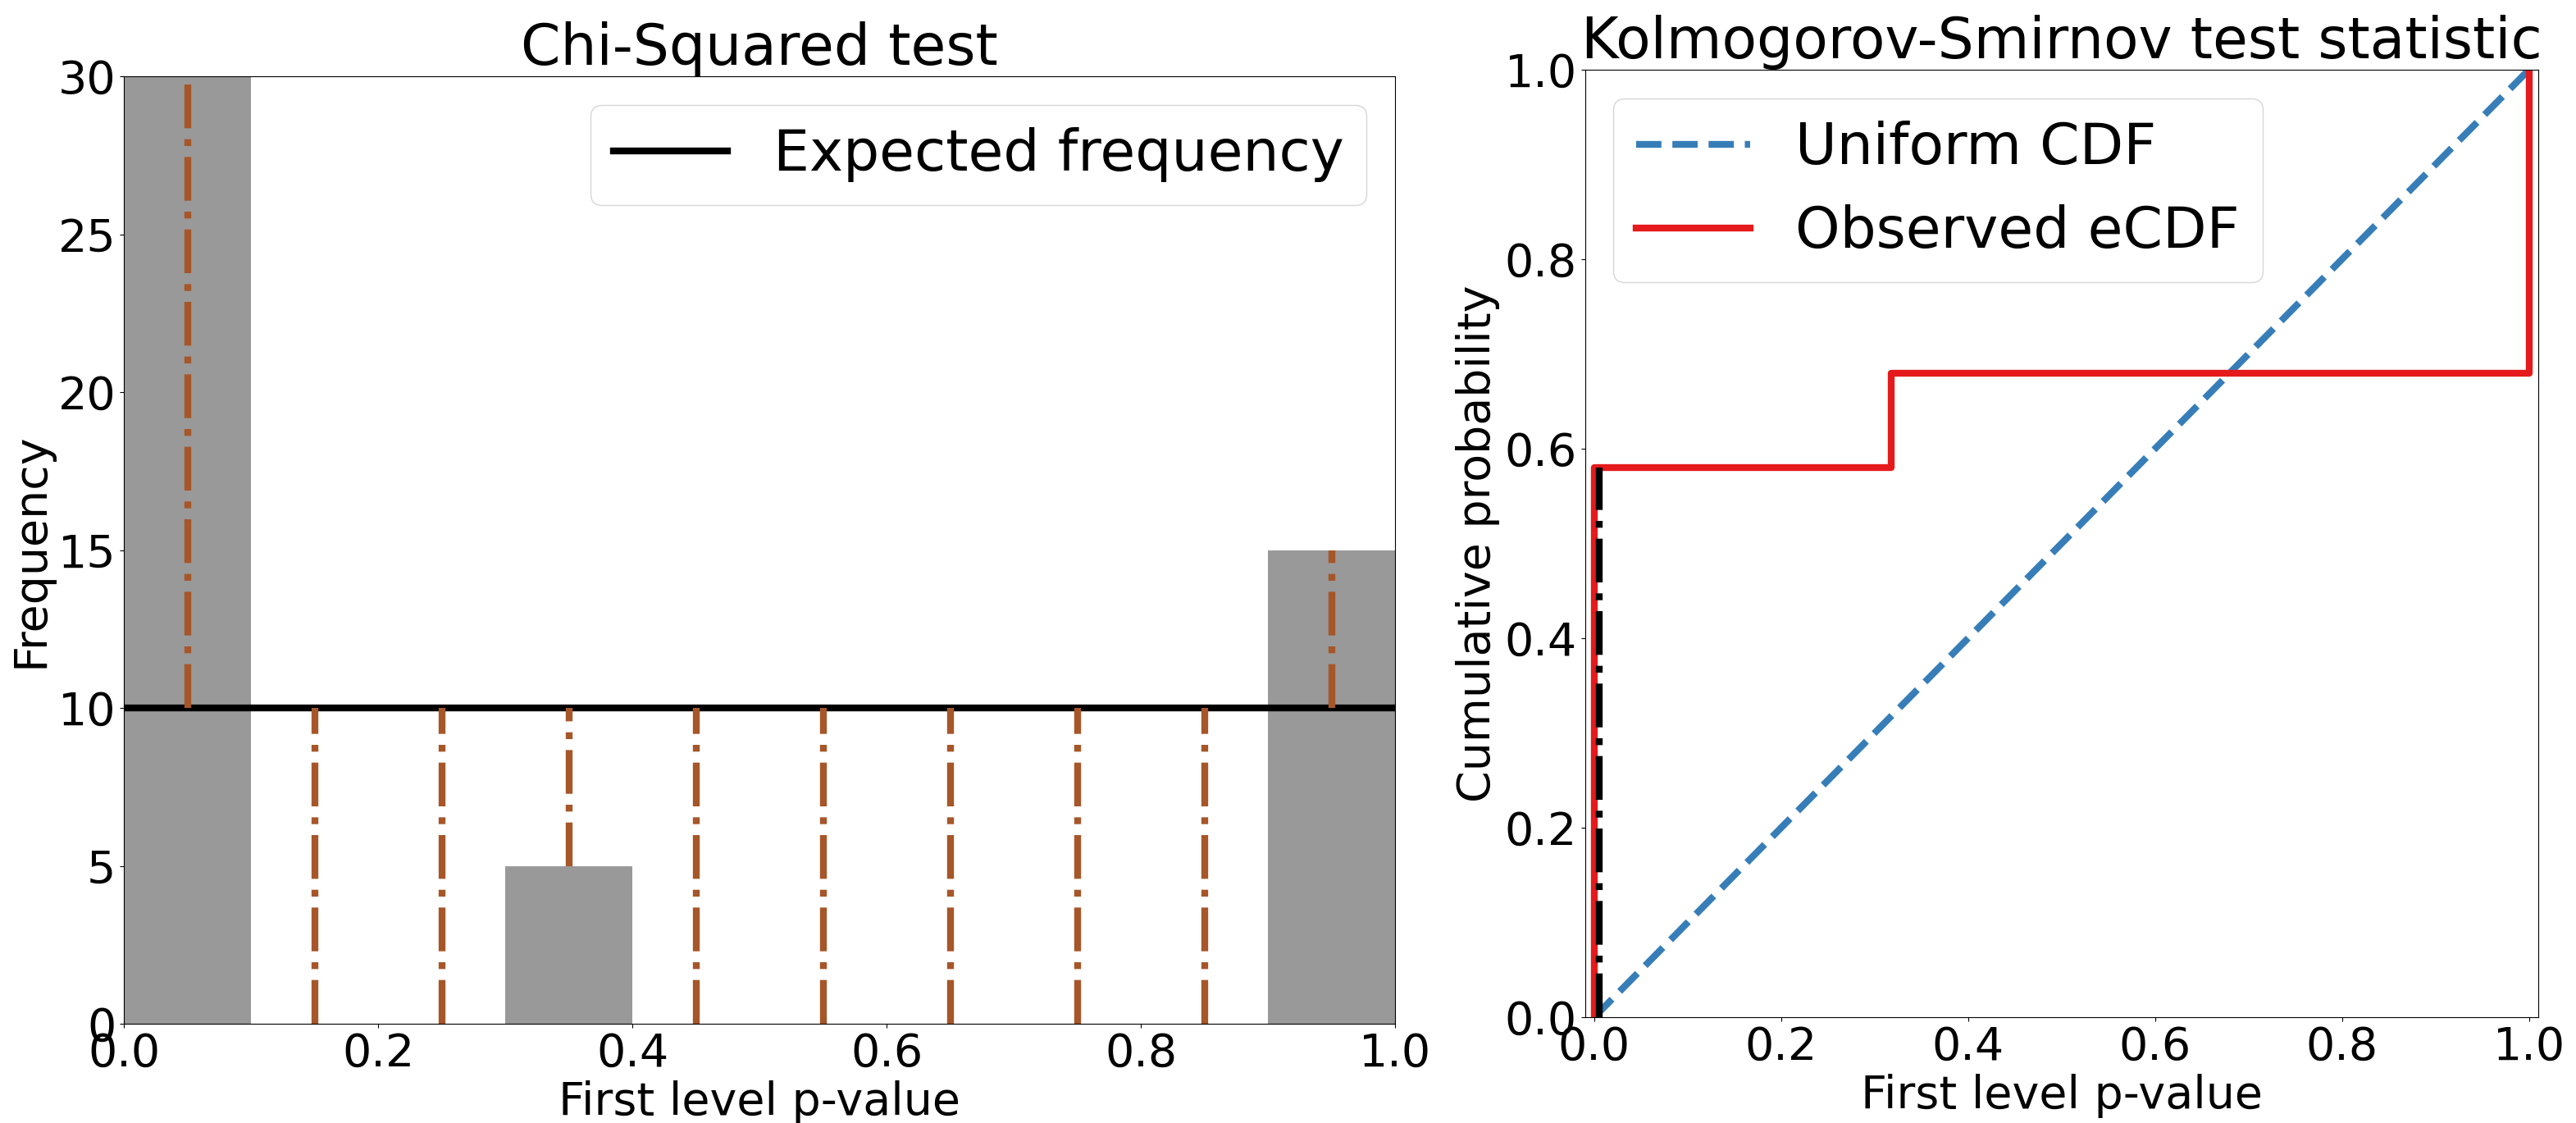
\includegraphics[width=13cm]{figures/two_example.png}
  \end{center}
  \caption{Visualisations for GOF tests example}
  \label{fig:two_example}
\end{figure}


% Old Chapter
\todo{DO NOT READ, WILL BE REMOVED}
\chapter{Randomness testing - old}

The goal of this chapter is to explain the mathematical background of randomness testing to the users of the \emph{Randomness Testing Toolkit} and make understanding of results and their deeper examination easier.

In the beginning, the motivation for randomness testing is presented. This is followed by overview of statistical testing process alongside the specifics of randomness testing. At the end, the two-level testing and use of goodness-of-fit tests are explained. Both of the explanations are accompanied by example execution of one test from practice. 

\section{Motivation}

Randomness testing is a form of empirical statistical hypothesis testing. During the test we want to find a proof supporting (or in the case of failure contradicting) the tested hypothesis. This is achieved by testing behaviour of the data set under the prediction that the tested hypothesis is true. When randomness is tested, the hypothesis states that the data are \emph{random}. This means that the data contain no patterns and thus each bit has exactly the same probability of being 1 or 0. The result of the test is either the acceptation of the hypothesis, or its rejection.

The tested data are streams of bits usually acquired from output of various cryptographic primitives, where randomness of the output is required or expected. These are usually (pseudo-)random number generators or ciphers. The randomness testing is then used to assess the quality of the data - whether the data are random, or if the data contain patterns (i.e. are non-random).

Each randomness test detects different set of patterns, therefore more tests are usually applied on the data at the same time. Groups of tests that are applied together are called test batteries. Some groups of test might also search for similar patterns in the data, therefore their results might be correlated. \cite[p. 2]{bad_day} TODO: MOVE TO RESULTS? In this case it is recommended to use more than only one group of tests.

\section{Process of testing} \label{chap:rand-process}

At the beginning of statistical testing, the tested \emph{null hypothesis}  ($H_0$) is set. Associated with the null hypothesis is the \emph{alternative hypothesis} ($H_1$) - the hypothesis we consider to be true in case the null hypothesis is rejected. In the case of randomness testing the null hypothesis states that the data are \emph{random} and the alternative hypothesis states that the data are not random.

Second step before we start the test is choosing the \emph{significance level} (usually denoted as $\alpha$). The chosen significance level is the probability of rejecting the null hypothesis in spite of the null hypothesis being true. The usual chosen values are $\alpha$ = 0.05 or $\alpha$ = 0.01. TODO: SOURCE, MAYBE ABOUT ALPHA ADJUSTMENTS

The last step is choosing the \emph{test statistic} (i.e. function of the data). This test statistic determines which kind of patterns are searched for in the current test. The test statistics vary in many different ways. There are test statistics based on simple sums of bits, but also statistics based on complicated transformations or statistics based on games. When choosing the test statistic, its distribution on random data must be known. TODO: SOMEWHERE MENTION THAT WE LOOK FOR TOO EXTREME SAMPLES

Once all of the previous have been chosen, the testing process begins. The process is started by obtaining data. During randomness testing these are taken from some source of randomness and are further viewed as a sequence of bits. Based on the test statistic, sequence with the required length is extracted and the rest of the data is discarded. Then the value of test statistic is computed and used to acquire the resulting \emph{p-value}. For more common distributions precomputed tables are available, for the remaining distributions the p-value must be computed.

The \emph{p-value} of the observed test statistic is the probability of drawing a test statistic value that is at least as extreme as the observed result. In other words, the p-value is sum of probabilities of test statistic values that are considered more extreme. The p-value can also be calculated as area under the probability density function (definite integral of this function) on interval of at least as extreme values.

There are three ways to determine what \emph{more extreme} value means. The first one is \emph{left (lower) tailed test}. In this case, more extreme values are all values lower than then observed value. The second one is the \emph{right (upper) tailed test}, where more extreme values are considered values greater than the observed values. Both of these variants are referred to as one-tailed tests.

The third way is the \emph{two-tailed test}, where more extreme values are found in both tails and the p-value therefore consists of two parts. The 'closer' tail is determined and then the fist part of p-value is computed as in one-tailed test. Then the second interval of more extreme values is established. This interval begins in the opposite tail and the area under the probability density function is equal to the first part of the p-value. Therefore it is not necessary to establish the second interval, because the second part of the p-value is equal to the first part. The p-value is either computed as sum of both of the parts or as double of the first part. 

The used approach depends on the executed test. For some test it is possible to use more than one approach only. At Figure \ref{fig:p_value} a visualization of all three approaches can be seen. In all cases, the value 2 was drawn from a standard distribution.

\begin{figure}
  \begin{center}
    %% minimus is about 100 pixels per 1 centimeter or 300 pixels per 1 inch.
    %% The optimum is about 250 pixels per 1 centimeter 
    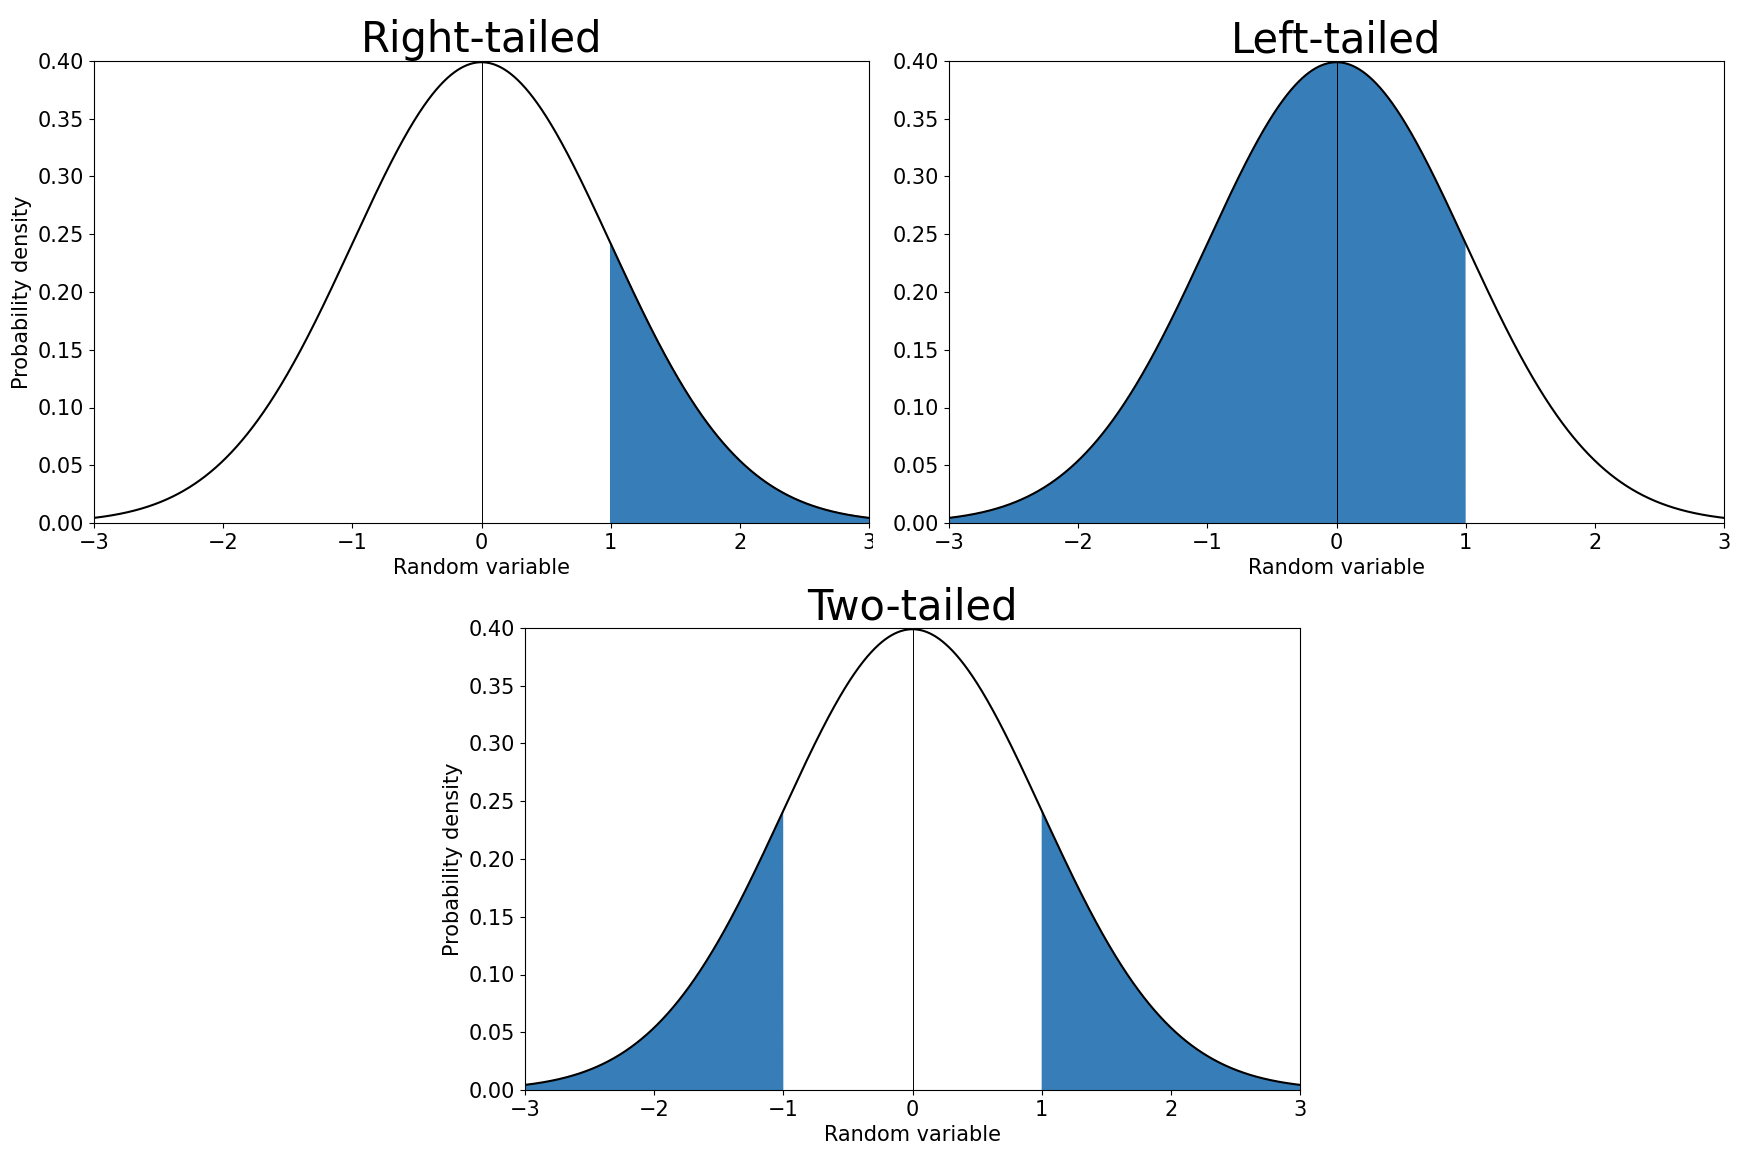
\includegraphics[width=12.5cm]{figures/p-value.png}
  \end{center}
  \caption{Visual interpretation of p-value }
  \label{fig:p_value}
\end{figure}

\section{Results interpretation} \label{chap:rand-interpretation}
TODO: SOME FIGURE WITH TWO OVVERLAPPING DISTRIBUTION

The test p-value is then used for interpretation of the test. If the p-value is less than the in advance chosen critical level, we consider the sample to come from a different distribution than is implied by the null hypothesis. In other words, the probability of drawing this sample in the distribution implied by the null hypothesis is so low, that it  we assume it must have come from a different distribution. Therefore, the null-hypothesis is \emph{rejected} and we consider the tested data to be \emph{non-random}.

If the \emph{p-value} is greater than the \emph{significance level}, no proof of the data being non-random was found and we \emph{accept} the null-hypothesis and consider the data to be \emph{random}.



However, the interpretation of results can be more than black and white only. In general, p-values close to the critical level can be considered \emph{suspicious}. Further analysis might then be in place. 

It is important to note that randomness testing is a \emph{statistical} testing. Therefore it is possible that the rejected (i.e. too extreme) sample was drawn only 'by chance'. Given that the null hypothesis stands, the probability of this happening is equal to the chosen \emph{significance level}.

\section{Example} \label{chap:rand-example}


To demonstrate how a single randomness test is made, the Frequency (Monobit) Test from NIST STS battery was chosen. \cite[p. 2-2]{nist_special} This is the simplest possible test, as it is based on testing the fraction of zeroes and ones within the sequence. For a random sequence $\epsilon$ with length $n$ the  count of ones is expected to be $n/2$ and is equal to expected count of zeroes.


It is easy to see that with one of the counts increasing (and the second one therefore decreasing), the sequence is getting less random. The probability of the bit being zero or one shifts from both being equal in favor of the more frequent bit.

For the Monobit, it is recommended that the tested sequence ($\epsilon$) has at least 100 bits. The test statistic of the Monobit test is defined as \[S_{obs} = \dfrac{|\#_1 - \#_0|}{\sqrt{n}}\] where $\#_1$ is count of ones in sequence $\epsilon$ (similarly for zeroes) and $n$ is length of of the sequence $\epsilon$. Under the null hypothesis, the reference distribution is half normal (for large $n$). The p-value is computed as \[ p = \int_{S_{obs}}^{\infty} F(x) \,dx = erfc(\dfrac{S_{obs}}{\sqrt{2}}) \] The $F(x) = \dfrac{\sqrt{2}\cdot e^{\frac{-x^2}{2}}}{\sqrt{\pi}}$ is the half normal distribution probability density function and $erfc$ is the \emph{complementary error function}.

 Let
\[\begin{split}
    \epsilon = 10011001010010000010001001011001101100001101000111\\10101001010010010011100111001100110010010100111011
\end{split}\]
 be the tested sequence. The test statistic for this sequence is 

 \[S_{obs} = \dfrac{|46 - 54|}{\sqrt{100}}\ = \dfrac{|-8|}{10} = 0.8\]
 and the p-value (visualised at Figure \ref{fig:example}) is 
 \[p = erfc(\dfrac{S_{obs}}{\sqrt{2}}) \doteq 0.423\]

At the end, we compare the computed \emph{p-value} to the chosen $\alpha$. Since the $\emph{p-value} \doteq 0.423$ is greater than both usual $\alpha = 0.05$ and $\alpha = 0.01$, we accept the null hypothesis for both \emph{significance levels}. Therefore, the sequence $\epsilon$ is considered random.

\begin{figure}
  \begin{center}
    %% minimus is about 100 pixels per 1 centimeter or 300 pixels per 1 inch.
    %% The optimum is about 250 pixels per 1 centimeter 
    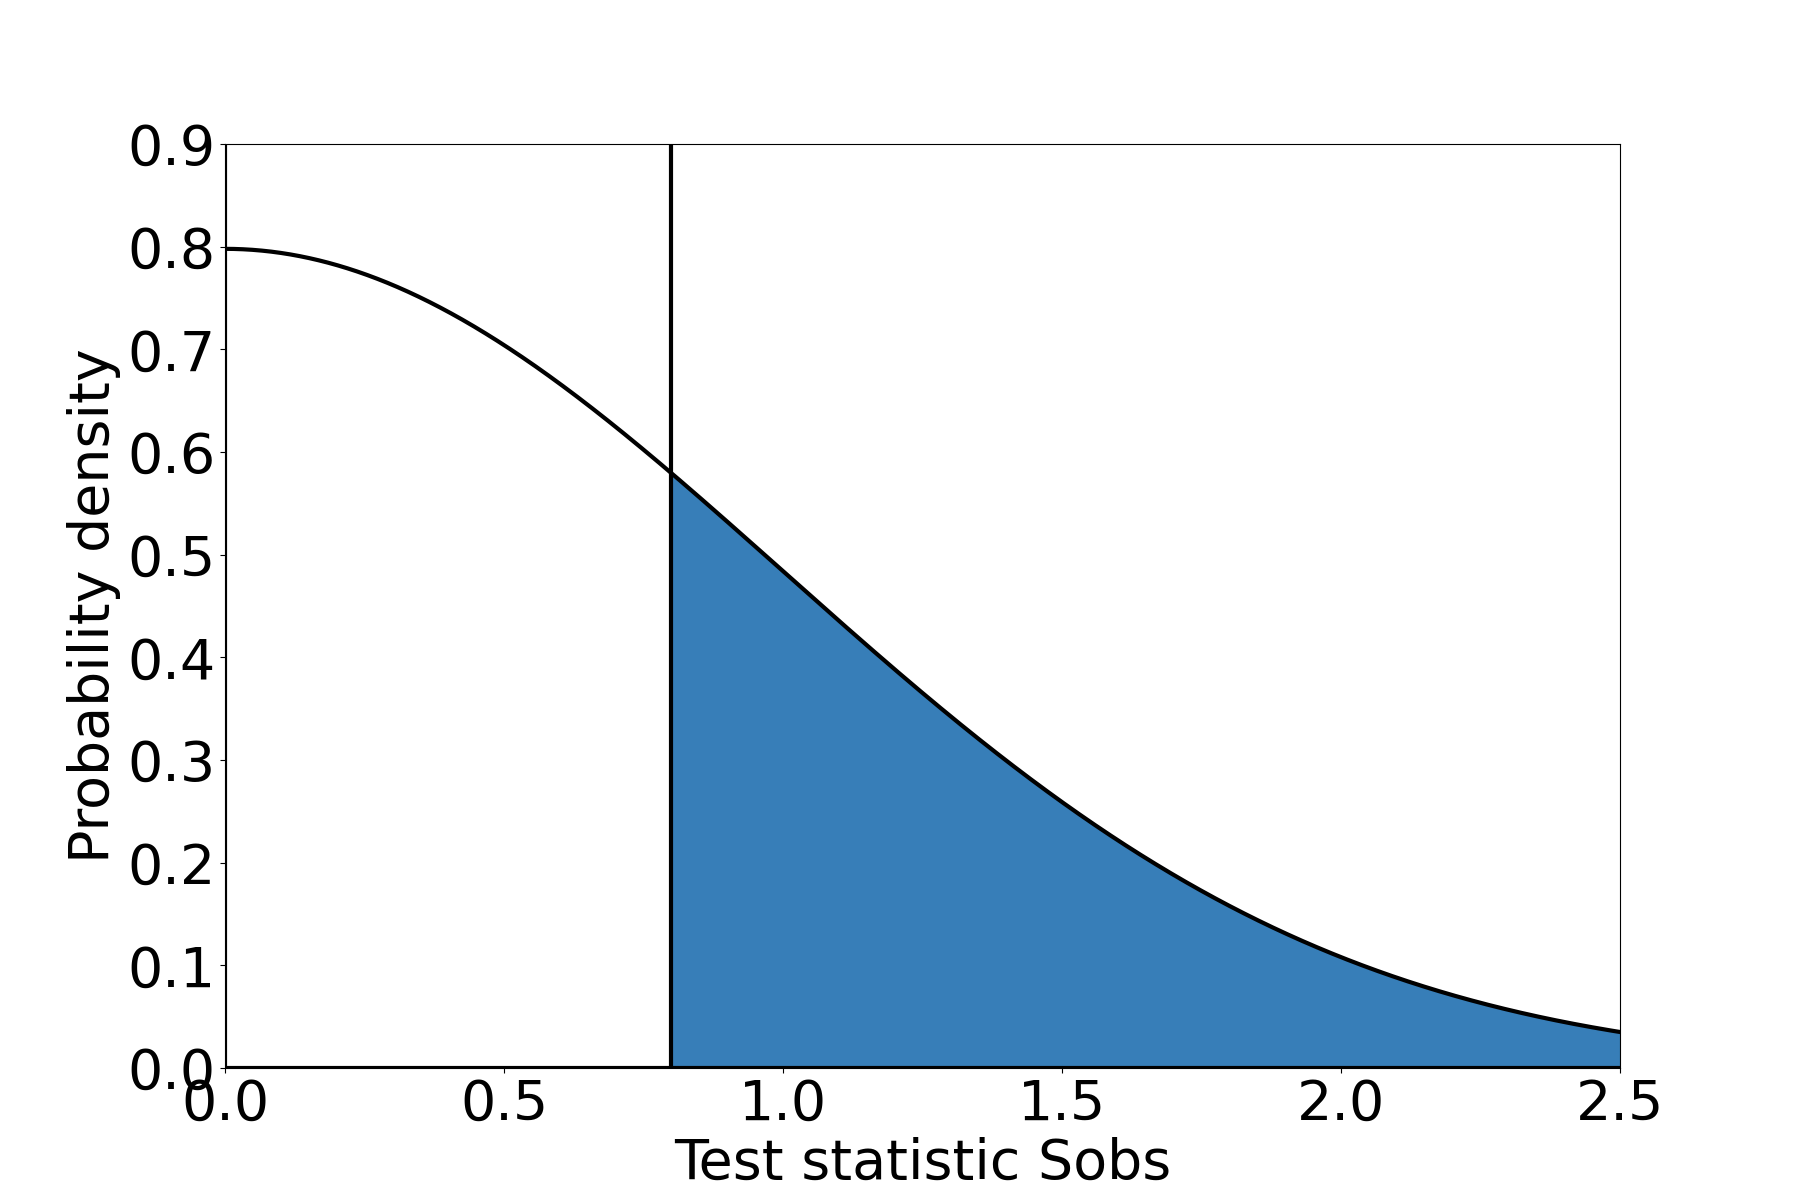
\includegraphics[width=8cm]{figures/test_example.png}
  \end{center}
  \caption{Visualization of example p-value}
  \label{fig:example}
\end{figure}

 



\section{Two level testing} \label{chap:rand-two_level}

TODO: mention expected fails of of first levels, figure with schema, mention remaining GOF tests


Two-level testing is used for a further examination of the data and can yield stronger information than using a one-level testing only. For example when we examine the sequence 
\[\begin{split}
    \epsilon =\:15\: &* (100\:consecutitive\:zeroes) + \\
    15\:&*\:(100\:alternating\:ones\:and\:zeroes) + \\
    5\:&*\:(55\:zeroes\:and\:45\:ones)\:+\:\\
    15\:&*\:(100\:consecutive\:ones)
\end{split}\]
it will pass the Monobit test (as used in Section \ref{chap:rand-example}) without raising suspicions of non-randomness with p-value $\doteq$ 0.479. However this sequence clearly contains a pattern and is not random. 

To perform a two level test, we split the original sequence into $n$ equal length non-overlapping sequences. Then we perform a standard statistical test as described in Section \ref{chap:rand-process} on each of these sequences in separate and collect all of the p-values they generated. These tests are then called first-level tests and their respective p-values are called first-level p-values. 

Note that the first-level p-values are not interpreted at this moment. It is in fact expected that some first-level p-values will be lower than the chosen \emph{significance level} (these would usually be considered failed). Given that the null hypothesis is true, the number of 'failed' first-level tests is expected to be $\alpha\cdot100\%$ of the total number of first-level p-values.

The first-level p-values are only treated as data in second round of testing, where goodness of fit tests are used - the second-level test. The goodness-of-fit tests are used to determine how well the observed data fit expected distribution. The most notable examples of tests from this category are the Kolmogorov-Smirnov test and the $\chi^2$ test, another examples are Cramér-von Mises test and Anderson-Darling test. 

For the first-level p-values a uniform distribution with interval $<0,1>$ is expected. The second-level test yields one second-level p-value, which is interpreted the same way a one-level test p-value would be (as described in Subsection \ref{chap:rand-interpretation}). Several goodness of fit tests can be applied at the same set of first-level p-values at once, because each test examines different uniformity properties of the data.

TODO: DIG DEEPER INTO DIFFERENCES BETWEEN GOF TESTS

% KS - description
\subsection{Kolmogorov-Smirnov test}
There are two variants of the Kolmogorov-Smirnov test (KS test). Two-sample test is used for comparing distributions of two data samples (to check if the data samples share the same distribution). The second variant, which is used in randomness testing, is the one-sample test. The one-sample test is used to compare a data sample against a theoretical distribution.

The Kolmogorov-Smirnov test is based on comparing the cumulative distribution function (CDF) of the expected distribution and the empirical cumulative distribution function (eCDF) of the observed samples. The Kolmogorov-Smirnov ($D$) statistic is the maximal absolute difference (vertical distance) between the expected CDF and observed eCDF (as can be seen in Figure \ref{fig:ks_d}). In some variants of the Kolmogorov-Smirnov test two statistics are measured - the maximal distance above the CDF ($D^+$) and the maximal distance below the CDF ($D^-$). Once the statistic is obtained, the second-level p-value is computed. Formally, the test statistics are defined as
\[\begin{split}
    &D^+ = sup_x\{F_n(x) - F(x)\}\\
    &D^- = sup_x\{F(x) - F_n(x)\}\\
    &D \:\:\:= sup_x\{|F_n(x) - F(x)|\} = max(D^+, D^-)
\end{split}
\] where $F(x)$ is the CDF and $F_n(x)$ is the  eCDF \cite[p. 100]{GOF-techniques}.

\begin{figure}
  \begin{center}
    %% minimus is about 100 pixels per 1 centimeter or 300 pixels per 1 inch.
    %% The optimum is about 250 pixels per 1 centimeter 
    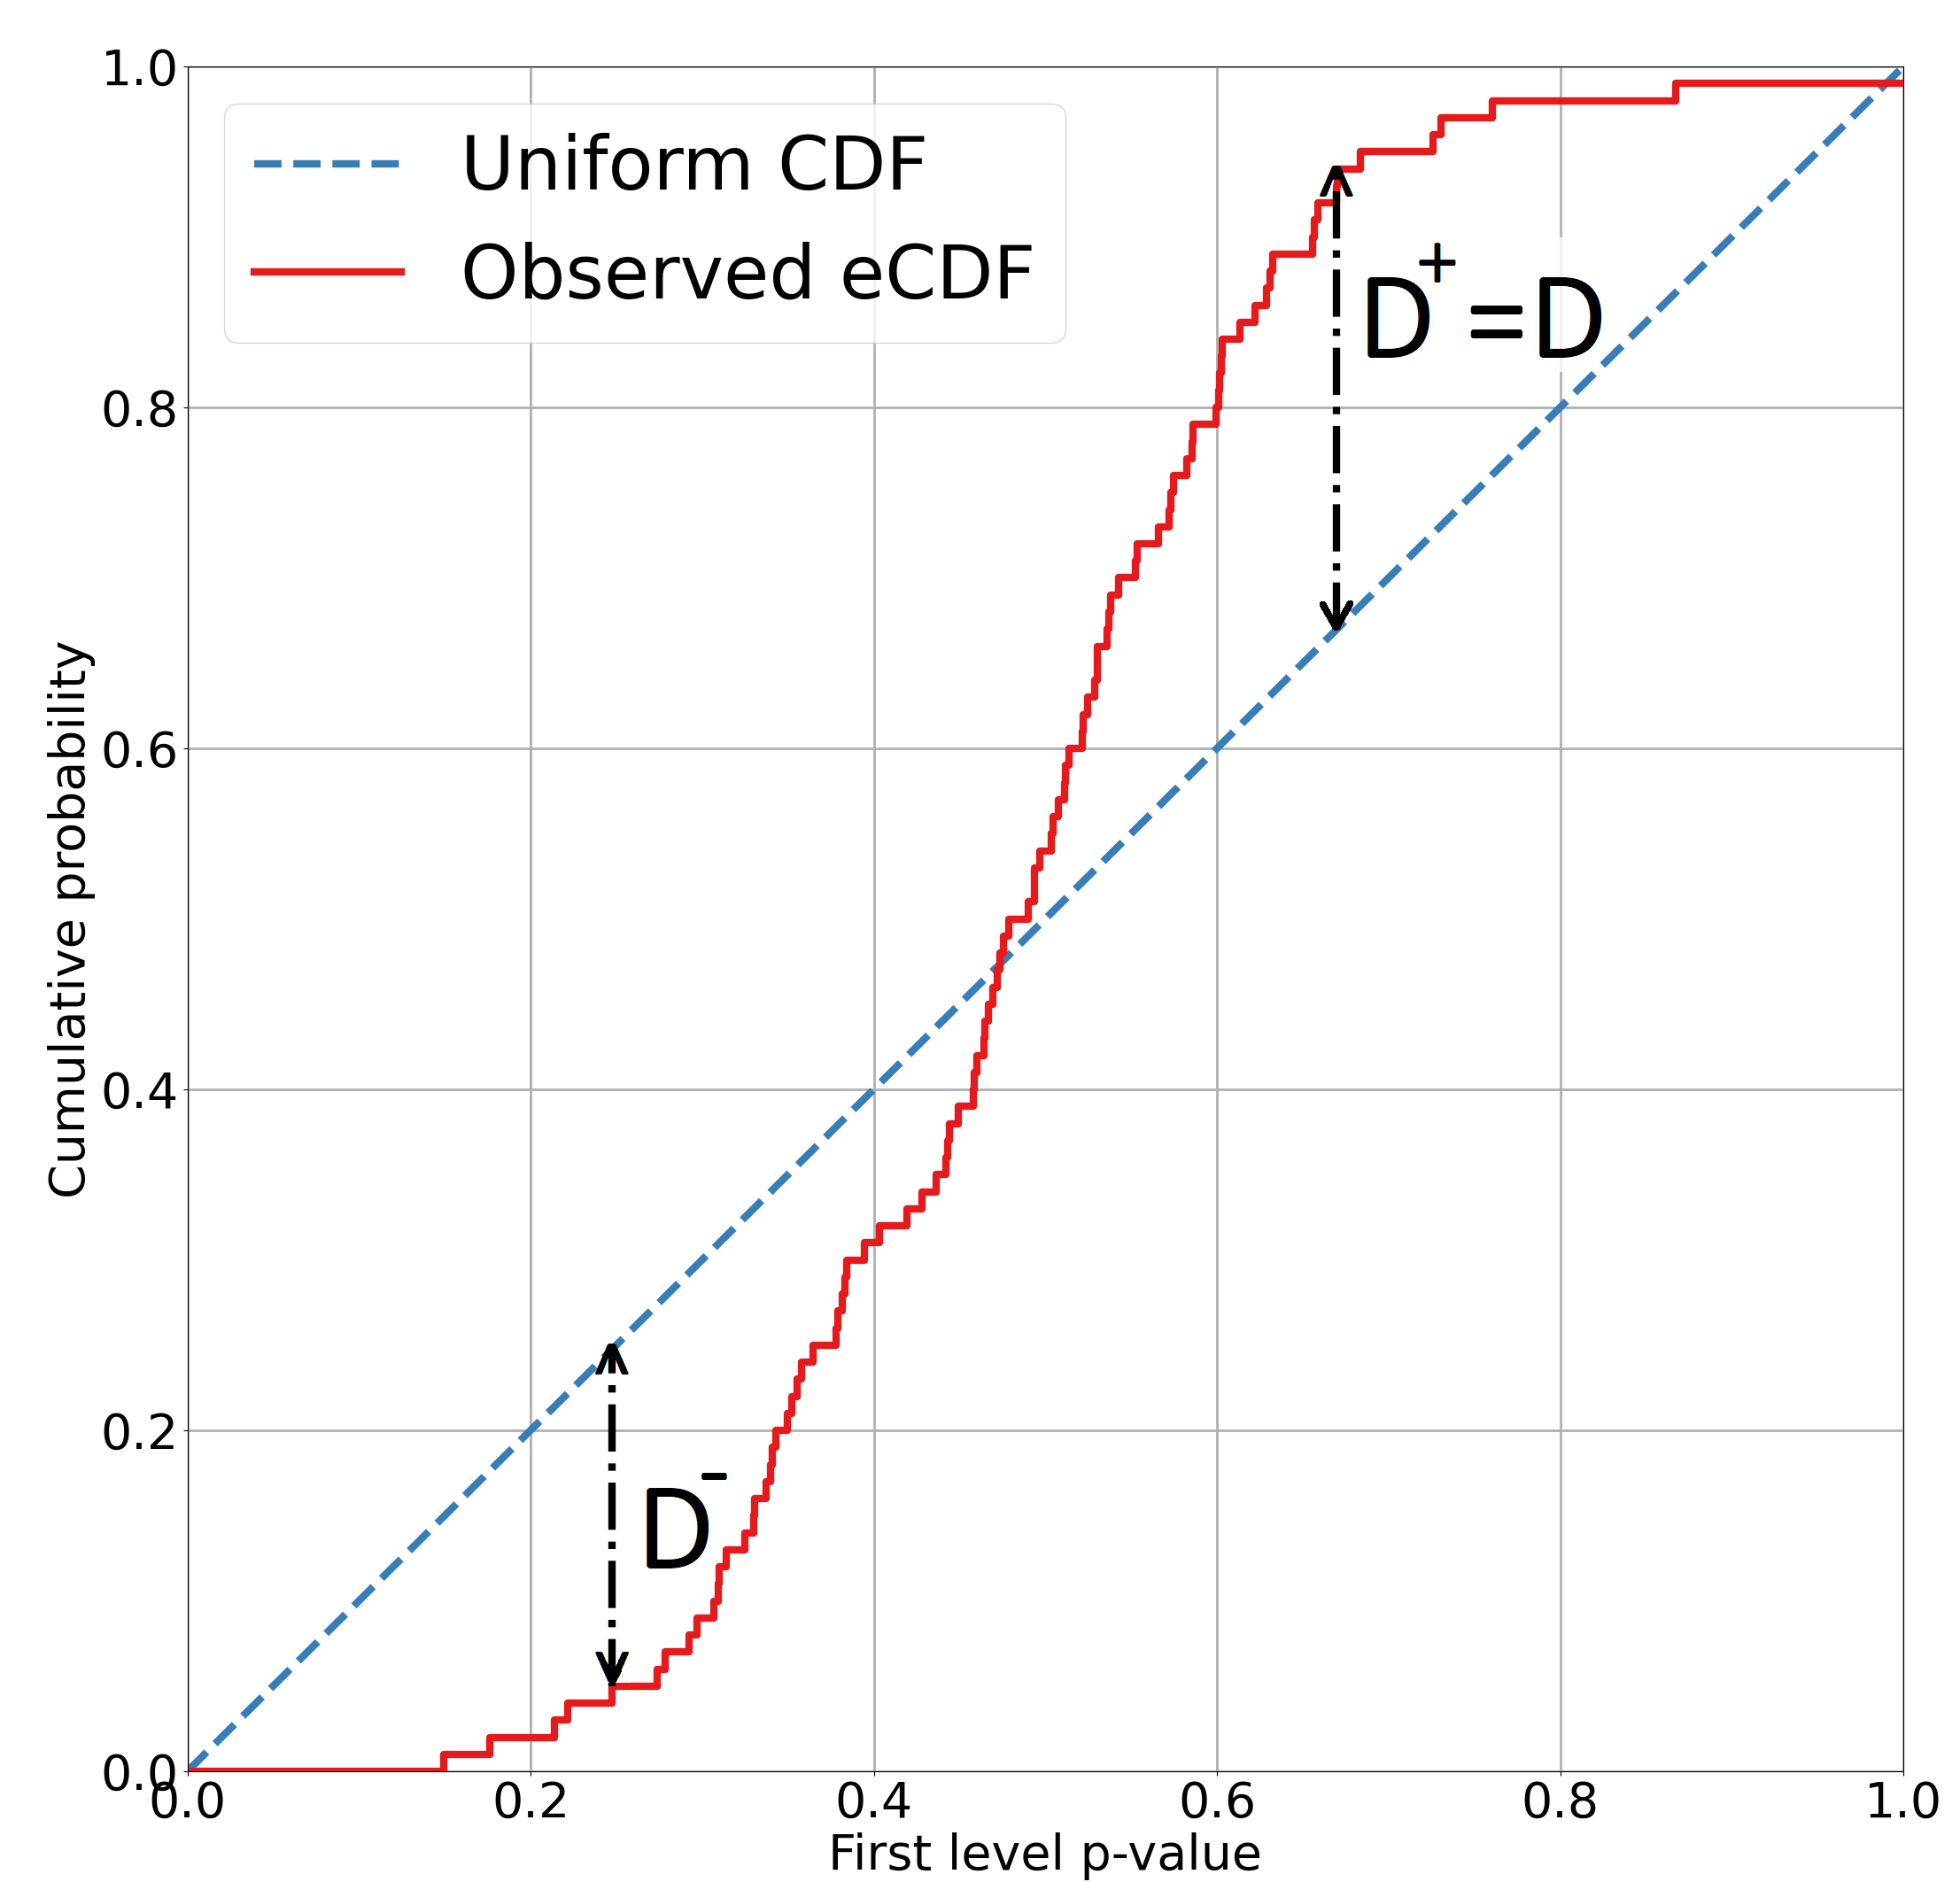
\includegraphics[width=8cm]{figures/ks_d.png}
  \end{center}
  \caption{Kolmogorov-Smirnov test statistics}
  \label{fig:ks_d}
\end{figure}


% $\chi^2$ description
\subsection{$\chi^2$ test}
$\chi^2$ tests are a group of several statistical tests used for comparing two sets of categorical data. The main one is the Pearson's $\chi^2$ test, that is used to determine existence of statistically significant difference in frequencies of categories in data sets. In randomness testing, one data set are the observed first-level p-values that are divided into $n$ equal-width categories and their respective frequencies are counted. The second data set are the expected frequencies for each category. Because the expected distribution of p-values is uniform, the expected frequencies are equal in each category. 
 
The test is based on summing squared differences in frequencies for each category between both sets of data. For data with $k$ categories the test statistic is defined as \[\chi^2 = \sum_{i=1}^{k} \dfrac{(x_i - m_i)^2}{m_i} \]
where $x_i$ is the observed frequency in $i$-th category and $m_i$ is the expected frequency in $i$-th category. The test statistic follows the $\chi^2$ distribution with $k-1$ degrees of freedom. The expected frequency in each category must be at least five. \cite[p. 171]{stat-procedures}
 
\subsection{Example}
\begin{table}
  \begin{tabularx}{0.4\textwidth}{ll}
    \toprule
    p-value & occurrences  \\
    \midrule
    $1.52 \cdot 10^{-23}$ & $30$\\
    $0.31$ & $5$\\
    $1.0$ & $15$\\
    \bottomrule
  \end{tabularx}
  \caption{First-level p-values produced by Monobit test}
  \label{tab:first_pvalues}
\end{table}



I will demonstrate the two-level test at example from the beginning of Section \ref{chap:rand-two_level}. As a first level test the Monobit \cite[p. 2-2]{nist_special} will be used to process subsequences with length of 100 bits. Because the length of sequence $\epsilon$ is 5000 bits, the first-level test will be run 50 times.

The sequence $\epsilon$ is now divided into 50 non-overlapping subseqeunces. The Monobit test is then applied to each subsequence  and its p-value is stored (for the obtained p-values see Table \ref{tab:first_pvalues}). It easy to see that these values are not uniformly distributed.

Next step is to apply one or more goodness of fit tests. The first one I will apply is the Pearson's $\chi^2$ test. I will choose $k=10$ (number of categories), the expected frequency of p-values in each category is then five. The statistic of the test is
\[\chi^2 = \sum_{i=1}^{10} \dfrac{(x_i - 5)^2}{5} = 180 \]
and the p-value of this test is $p\doteq5.06\cdot10^{-34}$. The null hypothesis is rejected for both $\alpha = 0.01$ and $\alpha = 0.05$. 

As next example, I will apply the Kolmogorov-Smirnov test. First, the eCDF is calculated and then the D statistic is computed. The statistic is $D = 0.6$ and results in p-value $\doteq$ $9.63\cdot10^{-18}$. Again, the null-hypothesis is rejected for both $\alpha = 0.01$ and $\alpha = 0.05$. 


\begin{figure}
  \begin{center}
    %% minimus is about 100 pixels per 1 centimeter or 300 pixels per 1 inch.
    %% The optimum is about 250 pixels per 1 centimeter 
    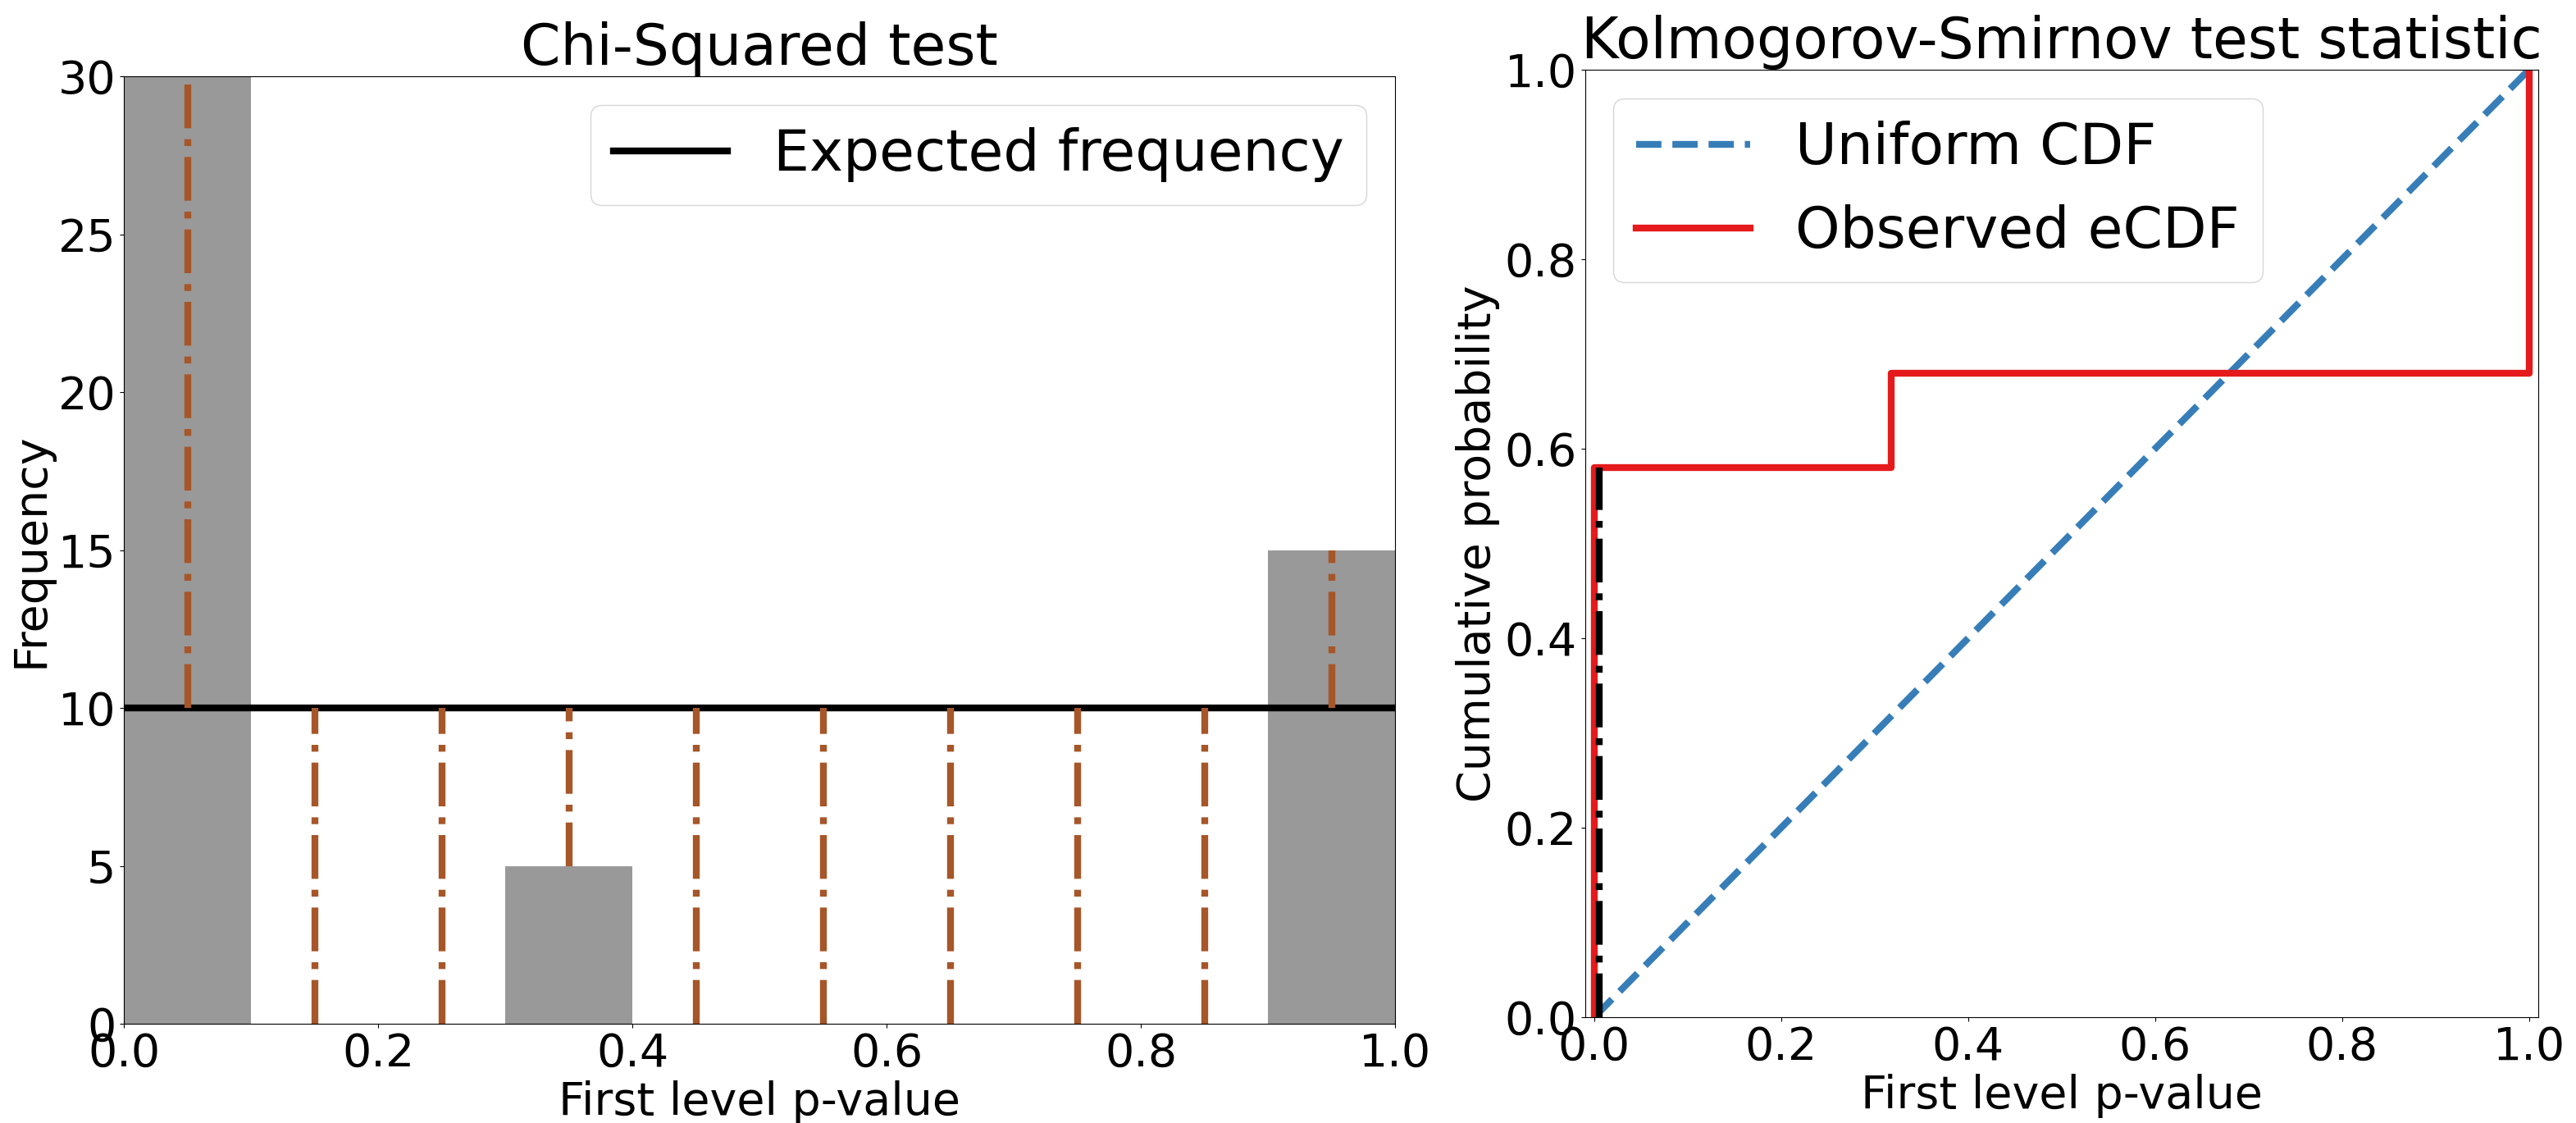
\includegraphics[width=13cm]{figures/two_example.png}
  \end{center}
  \caption{Visualisations for GOF tests example}
  \label{fig:two_example}
\end{figure}

%AVAILABLE SOLUTIONS

\chapter{Available solutions}


This chapter serves to describe various works and programs this thesis connects to. \\


\section{Statistical testing batteries}
More or less deep description of each battery. Should contain information about test parameters/settings.\\
\\
command on how to run battery\\
Mention overflow detection\\
If there are any problems with the battery (e.g. tests which read different amount of data from DieHarder). - Discuss colision with the paper\\

how batteries interpret results (first/second level, more statistics)\\
strong and weak things \\
describe output / image\\

\subsection{Dieharder}
Explain p-samples, name tests with irregular read bytes
\subsection{NIST STS}
Explain stream-size and stream-count\\
Results - in experiments directory

\subsection{Test U01}
List all batteries.
Explain repetitions, --bit -nb -w -r -s, mention repeating tests with different parameters


\section{Testing toolkits}\label{analysis}
JUST COPIED FROM WORK TO ACADEMIC WRITING COURSE, TO BE USED AND CHANGED LATER.\\

TODO: MENTION INSTALATION



In the previous chapter different randomness testing batteries were described. The typical user, however, uses more than one battery, which means installing and running each testing battery individually. Also it is strongly recommended (sometimes even needed) to set up parameters for each test from the battery individually based on tested file and to run this test manually.

Since this approach is not convenient, Ľubomír Obrátil from Center for Research on Cryptography and Security (CRoCS) at FI MU created the Randomness Testing Toolkit (\emph{RTT}). This toolkit allows users to run and configure three test batteries by a single command.

This work was followed by Patrik Vaverčák from Faculty of Electrical Engineering and Information Technology at Slovak University of Technology. He created newer variant of \emph{RTT} called Randomness Testing Toolkit in Python (\emph{rtt-py}). Compared to \emph{RTT}, it contains two additional test batteries. 

\section{Randomness Testing Toolkit}

\emph{RTT} was created in 2017 and its main idea was to combine \emph{Dieharder}, \emph{NIST STS}\footnote{National Institute of Standards and Technology - Statistical Test Suite} and \emph{Test U01} statistical test batteries into one program. It was written in C++. 

The concept of \emph{RTT} is that it acts only as a unified interface of the batteries. Each test battery is executed by \emph{RTT} as a separate program. The \emph{RTT} then collects the output and processes in into a unified format.~\cite[p.~8]{rtt-obratil}

However some problems in the processing of the output were found; these are addressed in chapter \ref{improvements}.

\subsection{Settings}\label{rtt-settings} 
TODO: MORE RIGID DESCRIPTION
The \emph{RTT} needs to be set up by the user before running. The first part of user settings contains general settings made for the \emph{RTT}, the second part contains configuration for individual test batteries. Each of these parts is stored in its own JSON\footnote{JavaScript Object Notation} file. The original setup description is from

The general settings are stored in \emph{rtt-settings.json} file, which has to be located in the working directory of the \emph{RTT}~\cite[p.~10]{rtt-obratil} . These settings are usually not changed between runs.
The most important setting from the general part are paths to the executable binaries of individual statistical test batteries. This is the only setting that has to be manually filled by the user.

The storage database can also be filled in by the user, but this functionality is often unused. The following general settings have implicit values and do no need to be changed unless the user wishes to. They are paths to storage directories for results and logs of individual runs and execution options (test timeout and maximal number of parallel executions of tests). 

 The battery configurations are dependant on the size of the tested file, therefore the file with the battery configuration is specified for each run of the \emph{RTT}. These configurations are different for each battery (see sections \ref{dieharder}, \ref{nist} and \ref{tu01}), but settings for all of the batteries can be stored together in a single file.~\cite[p.~11]{rtt-obratil}  The \emph{RTT} contains several prepared battery configurations for various sizes of tested file.



\subsection{Output}
The output of \emph{RTT} is in a plain text format. The most important part of the output is the direct report, which is saved in the results directory. At the beginning of the report are general information -- the name of the tested file, the name of the used battery, ratio of passed and failed tests and battery errors and warnings in case there were any.

After the general information is a list of results of individual test runs in a unified format. The fist part of the single test report contains the name of the test and user settings (\emph{e.g. P-sample count in Dieharder battery or Stream size and count in NIST STS battery}). The second part of the single test report are the resulting second-level P-values alongside the names of statistic used (usually Kolmogorov-Smirnov statistic or Chi-Square test). At the end of the single test report is a list of first-level P-values produced by the test. Example of the output can be seen in Figure \ref{fig:rtt_output_example}.

\begin{figure}
  \begin{center}
    %% minimus is about 100 pixels per 1 centimeter or 300 pixels per 1 inch.
    %% The optimum is about 250 pixels per 1 centimeter 
    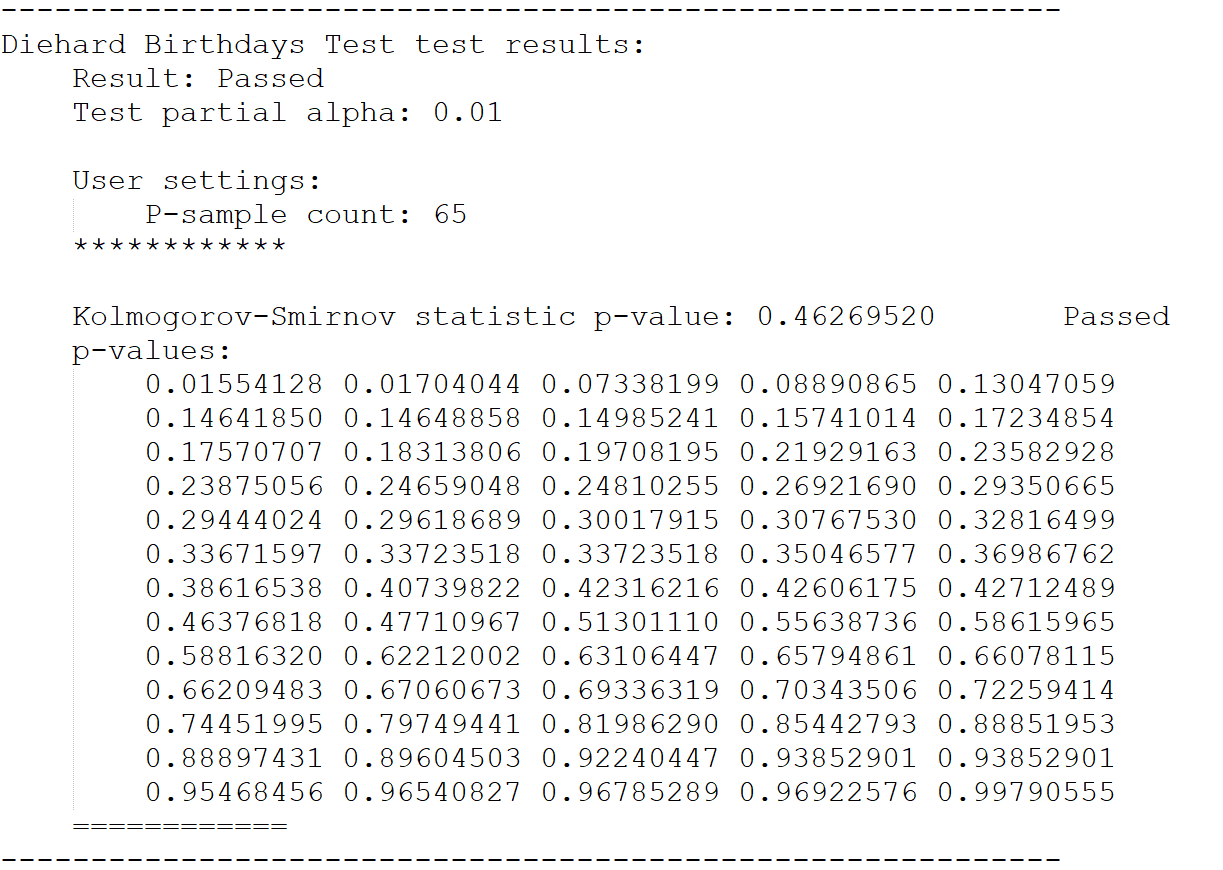
\includegraphics[width=12cm]{figures/rtt_dieharder_output.png}
  \end{center}
  \caption{The example of single test report from the \emph{RTT}}
  \label{fig:rtt_output_example}
\end{figure}

\subsection{Disadvantages}
The problems/weak points we want to improve with this thesis. Namely at least non machine-machine readable format, running only one battery at time, maybe re-calculation of results

There are two most notable disadvantages of the \emph{RTT}. The first one is that each battery has to be run individually by the user. This lowers the convenience of usage for the user. The second one is the output format. While it is easy to read for human users, machine reading requires complicated parsing. 



\section{Randomness Testing Toolking in Python}
The Randomness Testing Toolkit in Python (\emph{rtt-py}) was created by Patrik Vaverčák. It is supposed to be a better version of \emph{RTT}~\cite[p.~24]{vavercak} and it was written in Python. However there are still some functional differences between \emph{RTT} and \emph{rtt-py}. The most notable difference is in the output format and supported batteries.

\subsection{Settings}
The settings of \emph{rtt-py} are very similar to the original \emph{RTT}. According to Vaverčák, the general settings from the \emph{RTT} should be compatible with \emph{rtt-py}, but in reality there is problem with settings for the NIST STS's experiments directory. Also, no database connection is implemented in \emph{rtt-py}, therefore the \emph{mysql-db} attribute is ignored. \cite{rtt-py-github}


The second part of user settings are tests configurations. They use exactly the same format as those used in \emph{RTT} (as mentioned in \ref{rtt-settings}) and are interchangeable.~\cite[p.~25]{vavercak} The user has to keep in mind that the \emph{rtt-py} uses FIPS\footnote{Federal Information Processing Standards} and BSI\footnote{Bundesamt für Sicherheit in der Informationstechnik} batteries, which are not used in \emph{RTT}.

\subsection{Output}
There is a significant difference in the output format between \emph{RTT} and \emph{rtt-py}. The \emph{rtt-py} creates output in two formats -- \emph{CSV}\footnote{Comma-separated values} and \emph{HTML}\footnote{Hypertext Markup Language}. Both of these report formats contain overview table. Each row from the table represents results of one particular test. The first column contains the name of the test and the name of the battery it belongs to.

The second column contains \emph{failure rate} - ratio representing how many instances of this particular test failed compared to number of executed instances on \emph{all} files with data.


Each of the following columns is named after one tested file. The record contains either P-value reported by the test, or number of failed runs -- this depends on the battery. Example of this table can be seen at figure \ref{fig:rtt_py_table}.
\begin{figure}
  \begin{center}
    %% minimus is about 100 pixels per 1 centimeter or 300 pixels per 1 inch.
    %% The optimum is about 250 pixels per 1 centimeter 
    \frame{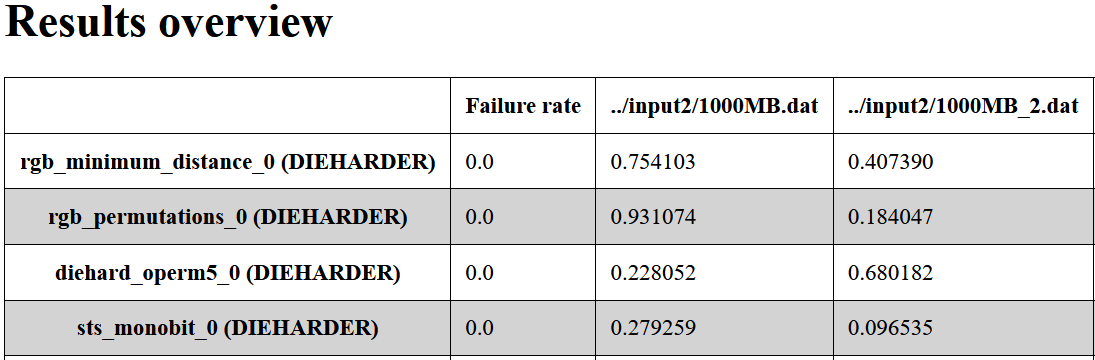
\includegraphics[width=14cm]{figures/rtt-py-table2.png}}
  \end{center}
  \caption{The example of the overview table from the \emph{rtt-py}}
  \label{fig:rtt_py_table}
\end{figure}


The output in the HTML format contains more information compared to the output in the CSV format. For each battery and for each tested file an HTML file with reports is generated.


In each report file there is a list of reports for each executed test from the given battery. The single test report contains the result of the test (either reported P-value, or number of failed runs) and it may contain additional information such as settings of the test or other information connected to the result. The contained information depends on the battery and on the executed test. Example of the  report can be seen in figure \ref{fig:rtt_py_html}
\begin{figure}
  \begin{center}
    %% minimus is about 100 pixels per 1 centimeter or 300 pixels per 1 inch.
    %% The optimum is about 250 pixels per 1 centimeter 
    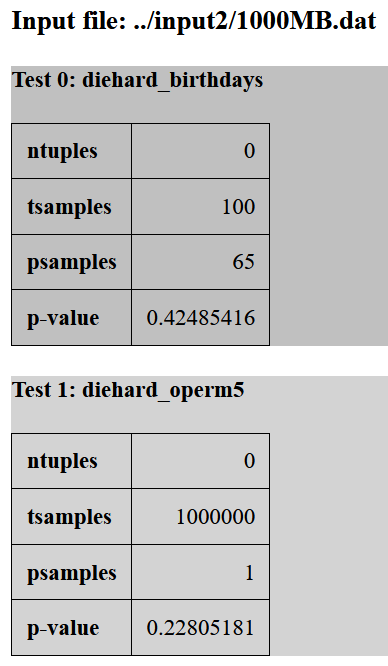
\includegraphics[width=6cm]{figures/rtt-py-dieharder-html.png}
  \end{center}
  \caption{The example of HTML Dieharder report from the \emph{rtt-py}}
  \label{fig:rtt_py_html}
\end{figure}

\subsection{Disdvantages}
One of the problems that need to be addressed is that the \emph{rtt-py } ignores errors and warnings from tests. The most notable example why this is a problem is when the tested file does not contain enough data for current battery configuration.

In this case, the test will read some parts of the data more than once and inform the user about this situation on the error output. The test will still produce result, which will, however, be biased by repeated parts of the tested file.

This may lead to incorrect interpretation of the results and to false acceptance or false rejection of the tested data. Since the \emph{rtt-py} ignores this, there is no way for the user to be informed about this situation.

Compared to the \emph{RTT} the reports created by \emph{rtt-py} contain less information. Namely the first-level P-values are ignored, even though they can be useful for deeper examination of the results and the generator.


% TEST ANALYSIS

\chapter{Tests Analysis}
We can choose from various test statistics. Most of the test statistics in widely used test batteries work with data of fixed length. TODO: REF ANALYSIS CHAPTER However, in some tests data with varying length are tested. These statistics further split into two categories. In the first category, the length of tested data is preset by user. These can be further viewed as fixed-length tests. In the second category, the length of tested data is determined during the testing process. 
\section{Data Consumption}
several big tables, mention exact parameters the tests  were run with

\section{Time Consumption}
again some big tables, choose one test as a reference and the rest will be relative. mention exact parameters, maybe add throughput?
\section{Configuration Calculator}
goal of the config calc, description, usage etc...
\section{P-Values}
Various problems with test p-values distributions, will probably be split into more sections



% IMPLEMENTATIONS COMPARISON
\chapter{Implementations Comparison}

\section{Output}
Mentioned differences\\
for both RTT and rtt-py - subset or whole?

\section{Missing Features of \emph{rtt-py}}

\section{Proposed improvements}
included things: adding first-level p-values, 

% CONCLUSION

\chapter{Conclusion}






\appendix %% Start the appendices.
\chapter{An appendix}
Here you can insert the appendices of your thesis.

\end{document}
